%results

\part{Results}
\label{sec:results}

\chapter{Golden Dual Fullerenes}
\label{sec:goldendualfullerenes}

\chapter[From Sticky-Hard-Sphere to Lennard-Jones-Type clusters]{
    From Sticky-Hard-Sphere to Lennard-Jones-Type clusters\footnote{This
    chapter is partly composed of sections previously published in the article
    ``From Sticky-Hard-sphere to Lennard-Jones-Type Clusters''\autocite{} and
    is reproduced with kind permission from the authors and APS (\textcopyright
    2018 American Physical Society).}
}
\label{sec:fromstickyhardspheretoLJtypeclusters}


%Introduction
\section{Introduction}


The nucleation of atoms and molecules in the gas phase, or liquid, to the solid
state is still an active research
field\autocite{Stillinger_Packingstructurestransitions_1984,
Martin-1996,Wales-1996, Vlieg_atomicscaleunderstandingcrystal_2007, Arkus-2010,
Woodley-2010, Karthika-2016, Holmes-Cerfon_StickySphereClusters_2017}.  Rowland
noted in 1949 that ``The gap between theory and the experimental approaches to
nucleation has been too wide'' and ``the subject [nucleation] is still in the
alchemical stage'' \autocite{Rowland-1949}. More than half a century later,
despite all the advancements made in cluster physics, ``there is still a large
gap between experiment and theory'' as Unwin noted \autocite{Unwin-2007}.

The underlying reason for this rather slow progress is that cluster formation
is a dynamic process, and fully characterizing the corresponding
high-dimensional potential energy landscape is typically an NP-hard problem,
since there are (presumably) exponentially many local minima at any given
temperature and pressure\autocite{Stillinger_Packingstructurestransitions_1984,
Oganov-2006, Massen_Powerlawdistributionsareas_2007, wales10, Oganov-2011,
calvo12, Wales-2015}.  Moreover, phase transitions between different
morphologies as a function of size $N$ usually occur where $N$ is too large for
an accurate quantum-theoretical treatment \autocite{Waal89,
Cleveland_energeticsstructurenickel_1991, vandewaal96a, Doye-1995,
vandeWaalTd00}.  For example, Krainyukova experimentally studied the growth of
argon clusters \autocite{Krainyukova-2012}, and found that small, initially
icosahedral clusters transform into anti-Mackay clusters for $N>2000$, and
finally into the \ac{fcc} or hcp structures at $N>10^5$ atoms, in
qualitative agreement with theoretical predictions using \ac{LJ} type
potentials \autocite{Martin-1996,
Schwerdtfeger_ExtensionLennardJonespotential_2006, Krainyukova-2007}.  The
notorious \textit{ rare gas problem} was solved only very recently by accurate
relativistic quantum methods, correctly predicting a slight preference of the
\ac{fcc} over the hcp phase due to phonon dispersion \autocite{Schwerdtfeger-2016}.

Simple models often have to be used to simulate cluster growth and nucleation
\autocite{Johnston-1999, Shibuta_Homogeneousnucleationmicrostructure_2015,
Leitold-2016, Sweatman-2016}.  The simplest model potentials that can be
applied to theoretical studies of atomic cluster formation are ``HCR-SRA''
potentials with isotropic hard-core-like repulsive and short-range-attractive
interactions \autocite{baxter68}.  The simplest HCR-SRA potential is the
``sticky hard sphere'' (SHS) potential \autocite{Yuste_Stickyhardspheres_1993}
\begin{align}
    V_\mathrm{SHS}(r)=\begin{cases}
        \infty, & r < r_s,\\
        -\varepsilon, & r = r_s,\\
        0, & r > r_s,
    \end{cases}
\label{eqn:KS}
\end{align}
where $r_s$ and $\varepsilon$ can be arbitrarily set to 1 (unit sphere and
reduced units, respectively).  Eq.~\ref{eqn:KS} can be used as a perturbative
basis for finite-ranged HCR-SRA potentials \autocite{cochran06,
Holmes-Cerfon_geometricalapproachcomputing_2013}.  Since sticky hard spheres
are impenetrable and their energy $E = -N_c\varepsilon$ ~is a function only of
the number of interparticle contacts $N_c$, SHS cluster structure and
energetics can be uniquely mapped to their adjacency matrices $\bar{A}$, where
$N_c=\sum_{i<j}^N A_{ij}$.  This mapping allows them to be exactly
characterized via complete enumeration
\autocite{Arkus_Minimalenergyclusters_2009, Arkus_DerivingFiniteSphere_2011,
Hoy_Structurefinitesphere_2012}; recent studies have identified all
mechanically stable SHS clusters for $N \leq 14$, and putatively complete sets
for $N \leq 19$ \autocite{Arkus_Minimalenergyclusters_2009,
Arkus_DerivingFiniteSphere_2011, Hoy_Structurefinitesphere_2012,
Hoy_Structuredynamicsmodel_2015, Holmes-Cerfon_StickySphereClusters_2017,
Kallus_Freeenergysingular_2017}.  Note, however, that different SHS structures
can have the same adjacency matrix for $N \geq 14$
\autocite{Holmes-Cerfon_EnumeratingRigidSphere_2016}, and the mapping is
therefore only surjective.

From the Gregory-Newton kissing-number argument proved in 1953 by Sch\"utte and
van der Waerden \autocite{Schutte_ProblemdreizehnKugeln_1952}, no sphere can be
surrounded by more than 12 spheres of equal radius \autocite{conway-2013book}.  For
small clusters, graph-theoretic arguments dictate $\mathrm{max}(N_c)\le
N(N-1)/2$.  Thus a loose bound on the maximum contact number $N_c(N)$ is
\begin{equation}
    N_c^\mathrm{max}(N) \le \mathrm{min}\{N(N-1)/2,f(N)\}
    \label{eqn:upperlimitNc}
\end{equation}
with $f(N)=6N$.  This upper bound has been tightened several times, most
recently by Bezdek and Reid \autocite{Bezdek-2013} to
\begin{equation}
    f(N)=6N-3(18)^{1/3}\pi^{-2/3}N^{2/3}.
    \label{eqn:upperlimitBR}
\end{equation}
In
Refs.~\autocite{Hoy_Structuredynamicsmodel_2015,Holmes-Cerfon_EnumeratingRigidSphere_2016}
it was shown that $N_c^\mathrm{max}(N) =
\{6,9,12,15,18,21,25,29,33,36,40,44,48,52,56,60\}$ for $4 \leq N \leq 19$.
While determining $N_c^\mathrm{max}(N)$ for arbitrary $N$ is equivalent to the
still-unsolved Erd\"os unit distance problem \autocite{Erdos-1946}, it is clear
that $N_c^\mathrm{max}(N) = 3N - 6 + m(N)$, where $m(N)$ grows slowly from zero
to around $f(N) - (3N-6)$ with increasing $N$.

While the maximum contact number increases (sub)linearly with $N$, the number of non-isomorphic cluster structures $|\mathcal{M}(N)|$ and 
transition states is assumed to increase exponentially \autocite{Stillinger_Exponentialmultiplicityinherent_1999,Oganov-2006,Forman_ModelingAggregationProcesses_2017} (here we denote $\mathcal{M}(N)$ as the set of all non-isomorphic cluster structures of size $N$, and 
$|\mathcal{M}(N)|$ as the number of structures in $\mathcal{M}(N)$).
Stillinger showed that under certain conditions $\lim_{N\to\infty} |\mathcal{M}(N)| \propto \exp(\alpha N)$ \autocite{Stillinger_Exponentialmultiplicityinherent_1999}.
For SHS clusters, the complete set $\mathcal{M}_\mathrm{SHS}(N,N_c)$ has been exactly
determined for $N \leq 14$ and $3N - 6 \leq N_c \leq N_c^\mathrm{max}(N)$ via exact
enumeration studies employing geometric rejection rules \autocite{Hoy_Structuredynamicsmodel_2015,Holmes-Cerfon_EnumeratingRigidSphere_2016}.
Unfortunately, such precise calculations are very difficult for finite-ranged
potentials since exhaustive searches for energy minima 
are computationally intensive \autocite{Heiles_Globaloptimizationclusters_2013}.  
Only a few such studies have been performed, e.g.\ recent studies of $N \leq 19$ clusters interacting via short-range Morse
potentials \autocite{wales10,calvo12,C7CP03346J}.

\begin{figure}\centering
    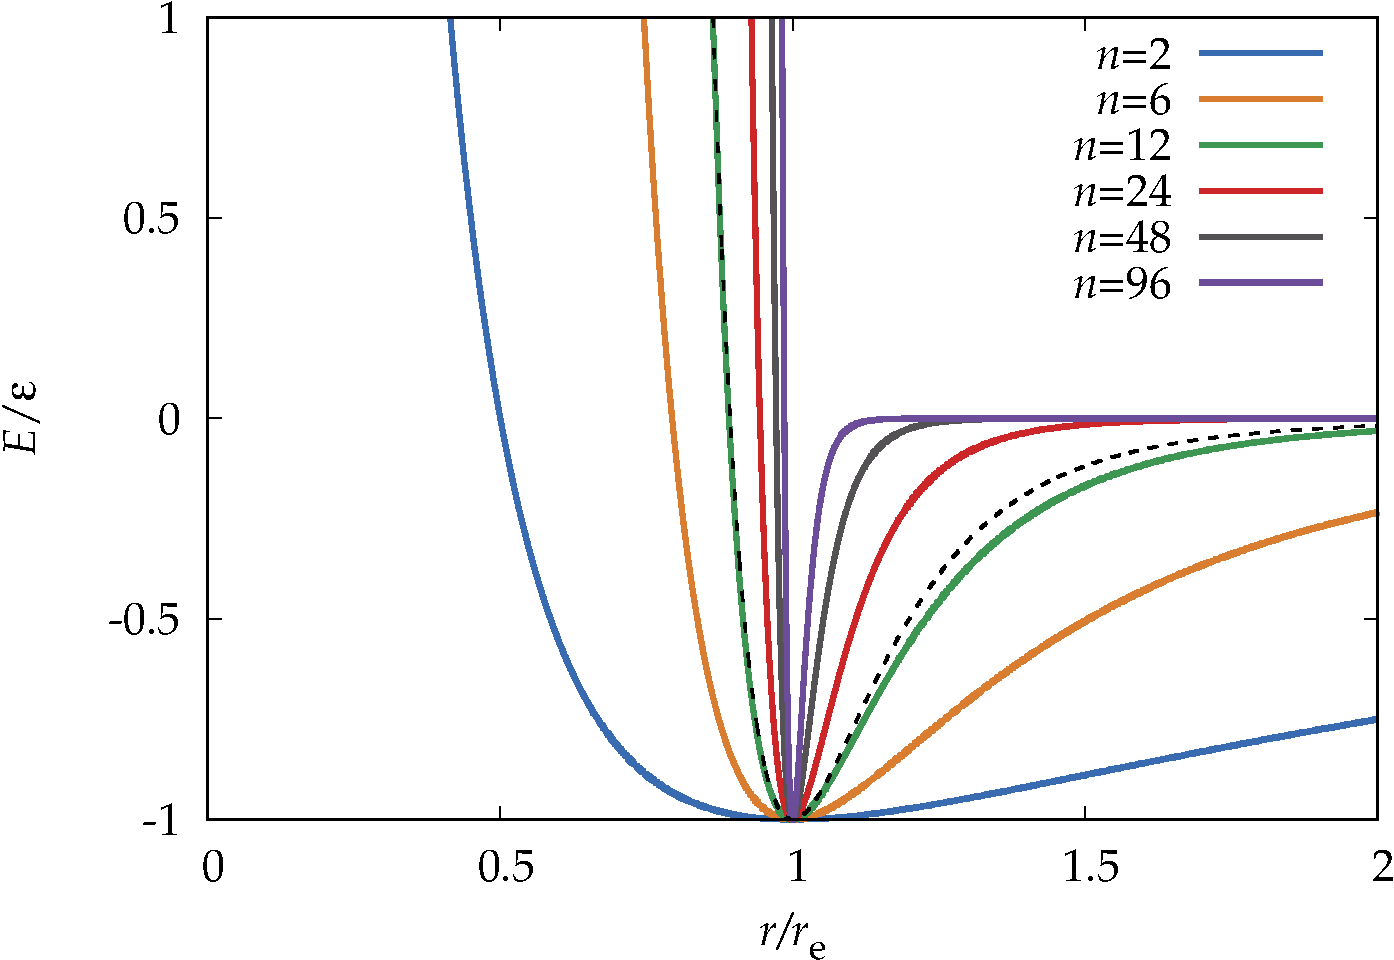
\includegraphics[width=0.8\columnwidth]{kslj/exampleLJ.pdf}
    \caption{Lennard-Jones potentials for different exponents $(m,n)$ with
    fixed $n=2m$. As the exponents grow larger the well of attraction becomes narrower 
    and its shape approaches the SHS potential. The dashed line
    shows the extended LJ potential for the xenon dimer \autocite{Jerabek_relativisticcoupledclusterinteraction_2017}.}
    \label{fig:LJ}
\end{figure}

It remains unclear how the HCR-SRA models commonly
used in cluster physics relate to more physically relevant, softer interaction potentials such
as the $(m,n)$-Lennard-Jones (LJ) form:
\begin{equation}
V_{m,n}^\mathrm{LJ}(r)=\frac{\varepsilon}{n-m}\left[m\left(\frac{r_e}{r}\right)^{n}-n\left(\frac{r_e}{r}\right)^{m}\right] \ \ \ \ \ \ \ \ \ \  ({\mathrm with}\ n > m).
\label{eqn:nmpot}
\end{equation}
Here $\varepsilon>0$ is the dissociation energy and $r_e$ the equilibrium
two-body interparticle distance. To simplify the presentation,
we (without loss of generality) adopt reduced units ($\varepsilon=1$, $r_e=1$) below.
For $m,n\rightarrow \infty$,
$V_{m,n}^\mathrm{LJ}(r) \rightarrow V_\mathrm{SHS}(r)$ (Fig.~\ref{fig:LJ}); the
energy landscapes of the two potentials converge in this limit.  However, real
systems are not in this limit.  For example, for $N = 13$, there are $|\mathcal{M}_\mathrm{SHS}|=97,221$
stable SHS clusters \autocite{Hoy_Structuredynamicsmodel_2015,Holmes-Cerfon_EnumeratingRigidSphere_2016},
but only $|\mathcal{M}_\mathrm{LJ}|=1,510$ stable $(m,n) = (6,12)$ LJ clusters \autocite{Doye_Evolutionpotentialenergy_1999}.  
This difference is understood qualitatively -- energy landscapes are well known to support more
local minima
as the range of the interaction potential decreases \autocite{braier90,Wales_MicroscopicBasisGlobal_2001}.
There are several effects that will cause the set of
stable LJ clusters to increasingly deviate from the set of stable SHS clusters
as interactions become longer ranged.  As $n$ and $m$ decrease,
second-nearest-neighbor attractions become increasingly important,
producing stable structures with $r_{ij} \leq 1$.  Fold catastrophes
\autocite{Wales_MicroscopicBasisGlobal_2001,wales04} progressively eliminate stable SHS clusters, and several stable SHS
structures may collapse into a single stable LJ cluster.  However,
detailed quantitative understanding of such effects remains rather limited.

In this paper, we quantitatively examine how stable $N \leq 14$ LJ cluster
structures evolve away from the SHS limit as ($m, n$) decrease.  We focus on
both the topography of the energy landscape (decreasing
$|\mathcal{M}_{\mathrm LJ}(N)|$) and the evolving topologies of the stable cluster sets.
We examine these changes in further detail for specific $N = 13-14$ clusters discussed by
Gregory and Newton in the 1600s in the context of the kissing number problem
\autocite{Schutte_ProblemdreizehnKugeln_1952}, and also for a more realistic two-body potential that has
been shown to accurately model rare-gas clusters \autocite{Schwerdtfeger_ExtensionLennardJonespotential_2006}.


%Computational Method
\section{Computational Methods}

The \textit{pele} program~\autocite{_pelePythonenergy_2017} was used to generate putatively
complete sets of local minima for $(m,n)$-Lennard-Jones potentials 
$V_{mn}^{\mathrm LJ}(r)$ as defined in Eq.(\ref{eqn:nmpot}).
This program  applies a basin-hopping algorithm that divides the potential energy
surface into basins of attraction, effectively mapping each point in
configuration space to a local minimum structure
\autocite{lis87,waless99,Wales_GlobalOptimizationBasinHopping_1997}.  The results confirmed the
number of local minima reported in previous work \autocite{Doye_Saddlepointsdynamics_2002}.
Finite computer time limited our search to clusters of size $N \leq 13$.

Starting from the sticky hard sphere packings up to $N=14$, with Cartesian
coordinates given by the exact enumeration algorithm \autocite{Hoy_Structurefinitesphere_2012}
including rigid hypostatic clusters ($N_c<3N-6$) \autocite{Holmes-Cerfon_EnumeratingRigidSphere_2016}, we carried out geometry
optimisations with $(m,n)$-Lennard-Jones potentials using the multidimensional function minimiser from the
\Cpp library \textit{dlib} \autocite{King_DlibmlMachineLearning_2009}. The optimisation scheme
was either the Broyden-Fletcher-Goldfarb-Shanno (BFGS) or the conjugate
gradient (CG) algorithm.  The optimisations were terminated when the change in
energy (in reduced units) over the course of one optimization cycle was smaller
than $10^{-15}$. 
Subsequently, the eigenvalues of the Hessian were checked
for all stationary points. If negative eigenvalues were found, the affected
structures were reoptimized following displacements in both directions along
the corresponding eigenvectors to locate true local minima. This procedure assures
that the floppy SHS packings are successfully mapped into LJ minima.

As the optimisations often result in many duplicates, especially for small
values of $n$ and $m$ where we have
$|\mathcal{M}_{(m,n)\mathrm{-LJ}}| \ll |\mathcal{M}_\mathrm{SHS}|$, the final
structures were further analysed and sorted. Nonisomorphic SHS clusters can be
distinguished (apart from permutation of the particles) by their different
adjacency matrices for $N \leq 13$ \autocite{Holmes-Cerfon_EnumeratingRigidSphere_2016}.  This is not the case for
soft potentials like the LJ potential since drawing edges (bonds) between the
vertices (atoms) becomes a matter of defining the distance cutoff criterion
for a bond to be drawn. Therefore, we compare the interparticle distances $\{r_{ij}\}$
instead: two clusters are isomorphic (structurally identical) if they have the same ordered
set of inter-particle distances $\{r_{ij}\}$.  While enantiomers cannot be
separated using this methodology, permutation-inversion isomers are usually
lumped together, since the number of distinct minima is analytically related to
the order of the corresponding point group \autocite{wales04}.  To verify the
number of distinct structures we introduced a second ordering scheme using the
energy and moment of inertia tensor eigenvalues. 

Two sets of structures are obtained from our optimization procedure: the first
set contains all possible LJ minima $\mathcal{M}_\mathrm{LJ}$ from the basin-hopping
algorithm, while the second set $\mathcal{M}_\mathrm{SHS\to LJ}$ contains the
LJ minima obtained using only the $\mathcal{M}_\mathrm{SHS}$ sticky-hard-sphere cluster structures as starting points for the geometry optimization.
To compare and identify corresponding structures between the two sets, the
$N(N-1)/2$ inter-particle distances $\{r_{ij}\}$ were again used as an identifying fingerprint.

Two-body ``extended Lennard-Jones'' (ELJ) potentials that accurately model two-body interactions in rare-gas clusters can be written as expansions of inverse-power-law terms \autocite{Schwerdtfeger_ExtensionLennardJonespotential_2006}:
\begin{equation} \label{eq:ELJ}
V_{\mathrm ELJ}(r)=\sum_{n} c_nr^{-n},
\end{equation}
where in reduced units the condition $\sum_{n} c_n=-1$ holds.
For comparison to the simple (6,12)-LJ potential, we used the ELJ potential
derived from relativistic coupled-cluster theory applied to the xenon dimer,
with the following coefficients for the ELJ potential (in reduced units):
$c_6=-1.0760222355$; $c_8=-1.4078314494$; $c_9=-185.6149933139$;
$c_{10}=+1951.8264493941$; $c_{11}=-8734.2286559729$;
$c_{12}=+22273.3203327203$; $c_{13}=-35826.8689874832$;
$c_{14}=+37676.9744744424$; $c_{15}=-25859.2842295062$;
$c_{16}=+11157.4331408911$; $c_{17}=-2745.9740079192$; $c_{18}=+293.9003309498$
\autocite{Jerabek_relativisticcoupledclusterinteraction_2017}. The ELJ potential for xenon is shown in
Figure \ref{fig:LJ} (dashed line).



%Results
\section{Results}

%Exploring the limits of Lennard-Jones
\subsection{Exploring the limits of Lennard-Jones}

To study the convergence behaviour of the number of distinct (nonisomorphic) LJ minima in
the SHS limit, we performed geometry optimisations,
starting from all nonisomorphic SHS structures.  We will show later that the
number of unique minima obtained in this procedure $|\mathcal{M}_\mathrm{SHS\to
LJ}|$ only misses out on a small portion of minima obtained from the more exhaustive
basin-hopping approach, i.e.~$|\mathcal{M}_\mathrm{SHS\to
LJ}|\approx|\mathcal{M}_\mathrm{LJ}|$.  The results for a constant chosen ratio
of LJ exponents $n/m=2$ are shown in Figure~\ref{fig:expinfty} (top). 
\begin{figure}
    \centering
    \subfloat{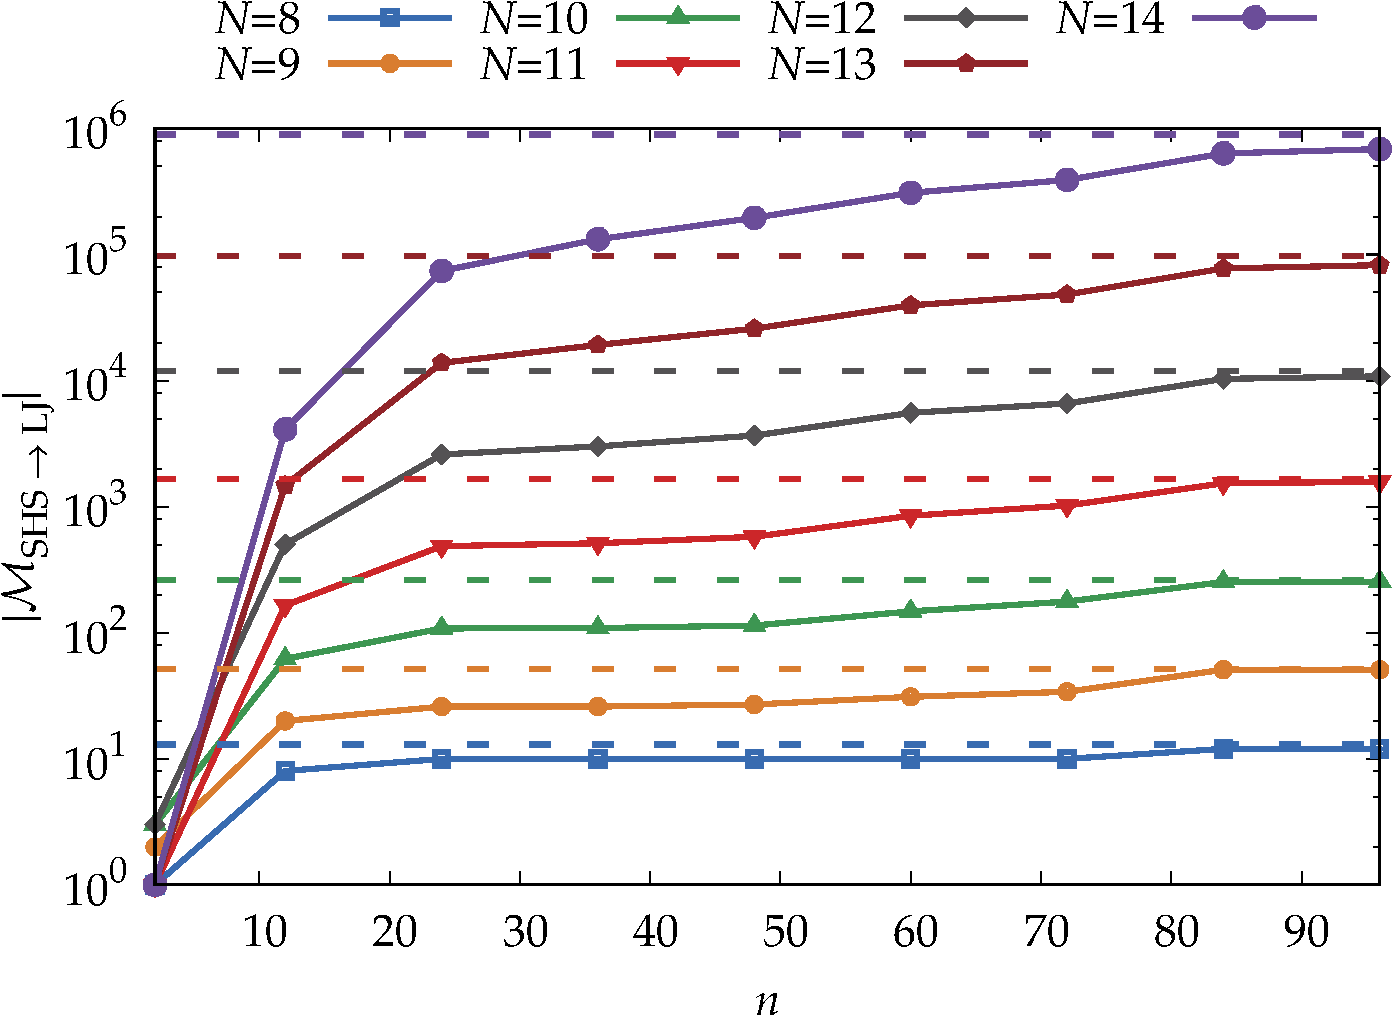
\includegraphics[width=0.8\columnwidth]{kslj/expinfty.pdf}}\\
    \subfloat{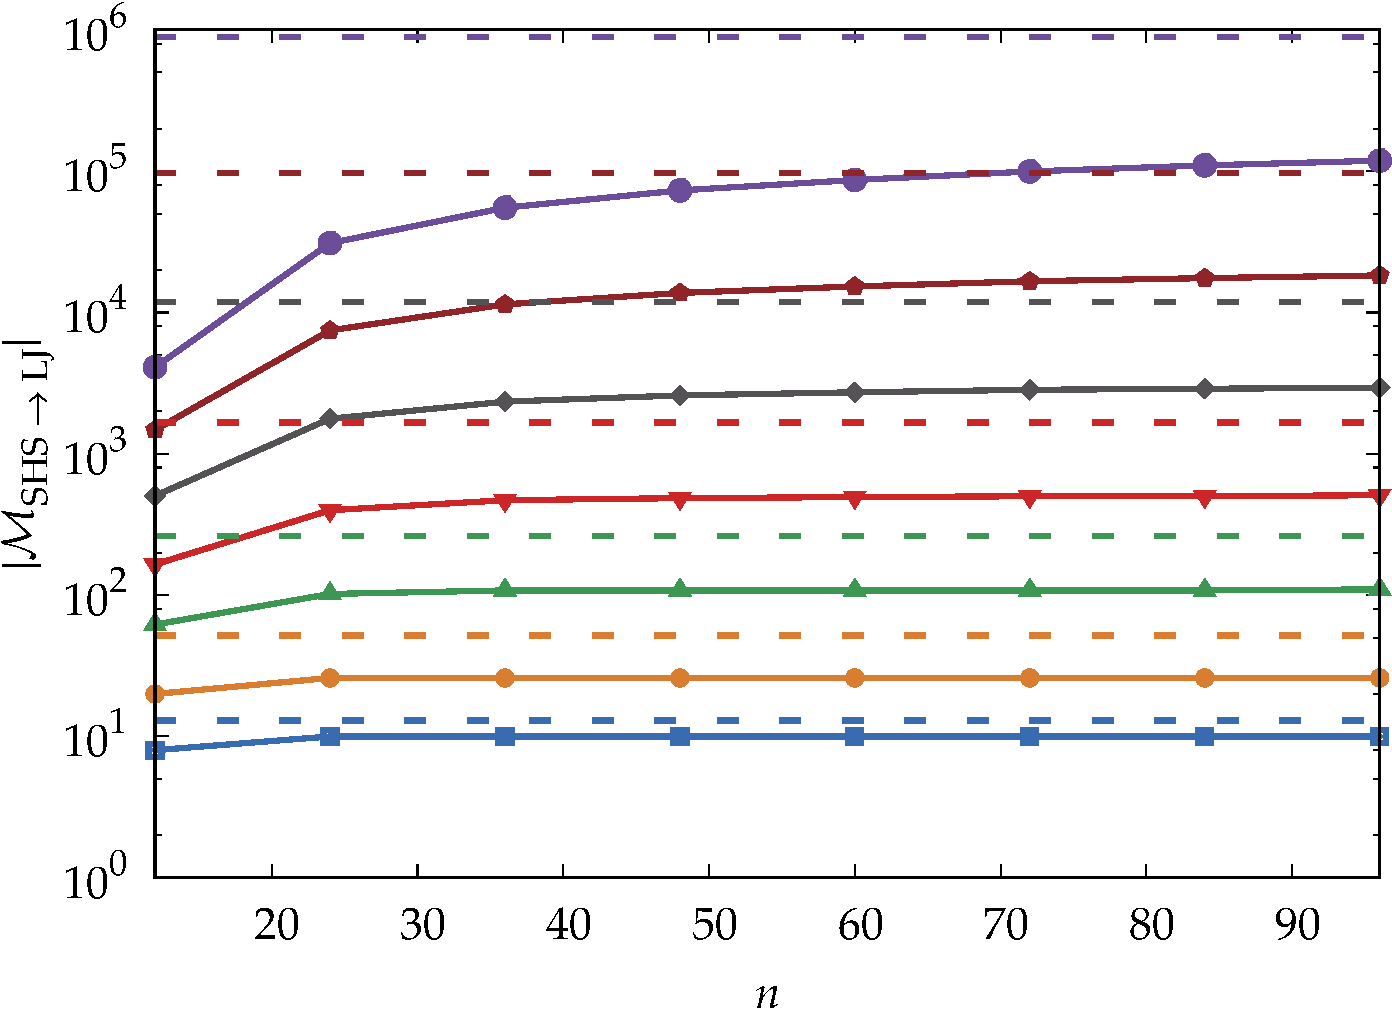
\includegraphics[width=0.8\columnwidth]{kslj/repulsive.pdf}}
    \caption{
    Convergence of the number of distinct LJ local minima
 $|\mathcal{M}_\mathrm{SHS\to LJ}|$
     obtained through geometry optimisations starting from the nonisomorphic SHS structures with
     increasing LJ exponent $n$. 
Permutation-inversion isomers and enantiomers are not distinguished.     
     The dashed line gives the exact SHS limit $|\mathcal{M}_\mathrm{SHS}|$. 
     Top panel: $m=n/2$. Bottom panel: fixed $m=6$.}
    \label{fig:expinfty}
\end{figure}

$|\mathcal{M}_\mathrm{SHS\to LJ}|$ smoothly  converges towards the SHS limit (dashed line, values in Table \ref{tab:comp}) from below, 
thus demonstrating that for LJ systems the number of distinct minima does not grow faster than exponentially.  
The (48,96)-LJ potential has $\Delta\mathcal{M} \equiv |\mathcal{M}_\mathrm{LJ}| - |\mathcal{M}_\mathrm{SHS\to LJ}| = \{1,1,7,91,1019,14890,209938\}$ fewer stable minima than the SHS potential.
The fractions of missing minima $\Delta\mathcal{M}/|\mathcal{M}_\mathrm{SHS}|$ for this potential grow with increasing $N$ and are respectively $\{7.69,1.92,2.67,5.46,8.62,15.32,23.44\}\%$.  Note that for $N \geq 10$ most of these missing minima correspond to high energy ($N_c < N_c^\mathrm{max}$) structures.


If the exponent $n$ for the repulsive part of the LJ potential is increased
with $m$ kept constant, the LJ potential becomes equivalent to the SHS
potential in the repulsive range but remains attractive at long range.
Figure~\ref{fig:expinfty} (bottom) shows the convergence of the number of
unique structures with respect to $n$ at set $m=6$ towards the SHS limit. Here, the
number of distinct minima converges towards a number that is much smaller
than the total number of SHS packings demonstrating that (as expected) the
attractive part of the potential contributes significantly to the decrease of
the number of local minima compared to the rigid SHS model.

To see if the asymptotic increase in the number of distinct minima $|\mathcal{M}(N)| \sim e^{\alpha N}$ 
is indeed exponential, we use Stillinger's expression for the asymptotic exponential rise rate parameter \autocite{Stillinger_Exponentialmultiplicityinherent_1999}
\begin{equation} \label{eq:Stil}
\alpha = \lim_{N\rightarrow \infty} \left( N^{-1} \mathrm{ln} |\mathcal{M}(N)| \right).
\end{equation}
Figure \ref{fig:asympt} shows the number of distinct minima for SHS clusters
obtained from the data shown in Table \ref{tab:comp}.  The $N \geq 12$ SHS data
gives $\alpha_\mathrm{SHS}\approx 2.21$. Figure \ref{fig:asympt} also shows the
(6,12)-LJ results obtained using basin-hopping; these yield
$\alpha_\mathrm{LJ}\approx 1.10$, which is close to the $\alpha=0.8$ value
estimated by Wallace \autocite{Wallace-1997} or to the recently given value of 1.04
by Forman and Cameron \autocite{Forman_ModelingAggregationProcesses_2017}.  Note that the rapid increase of
$|\mathcal{M}_\mathrm{SHS}|/|\mathcal{M}_\mathrm{LJ}|$ with $N$ is explained by
the much larger values of $\alpha$ for the SHS compared to the LJ clusters.

\begin{figure}
    \centering
    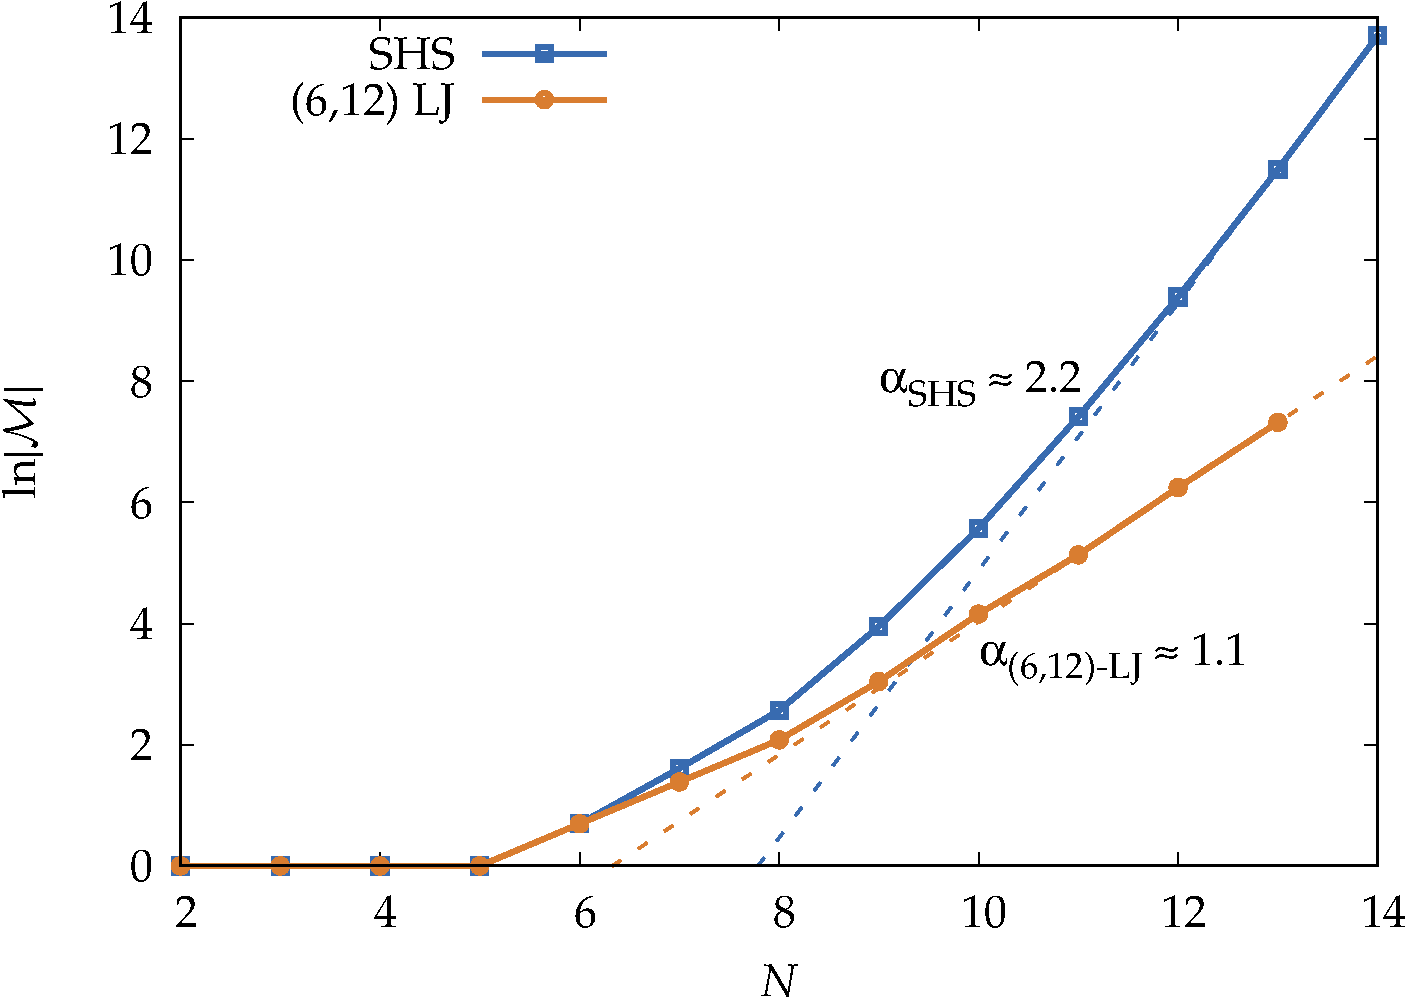
\includegraphics[width=0.8\columnwidth]{kslj/growth.pdf}
    \caption{Growth behaviour of $|\mathcal{M}(N)|$ of SHS and (6,12)-LJ clusters and 
    corresponding asymptotic exponential rise rate parameter $\alpha$ for $N \geq 12$ as defined in Eq.(\ref{eq:Stil}).
    The intercepts ln$|\mathcal{M}(N=0)|$ are $-17.19$ and $-6.94$ for the SHS and (6,12)-LJ cases respectively.}
    \label{fig:asympt}
\end{figure}

\begin{figure}
    \centering
    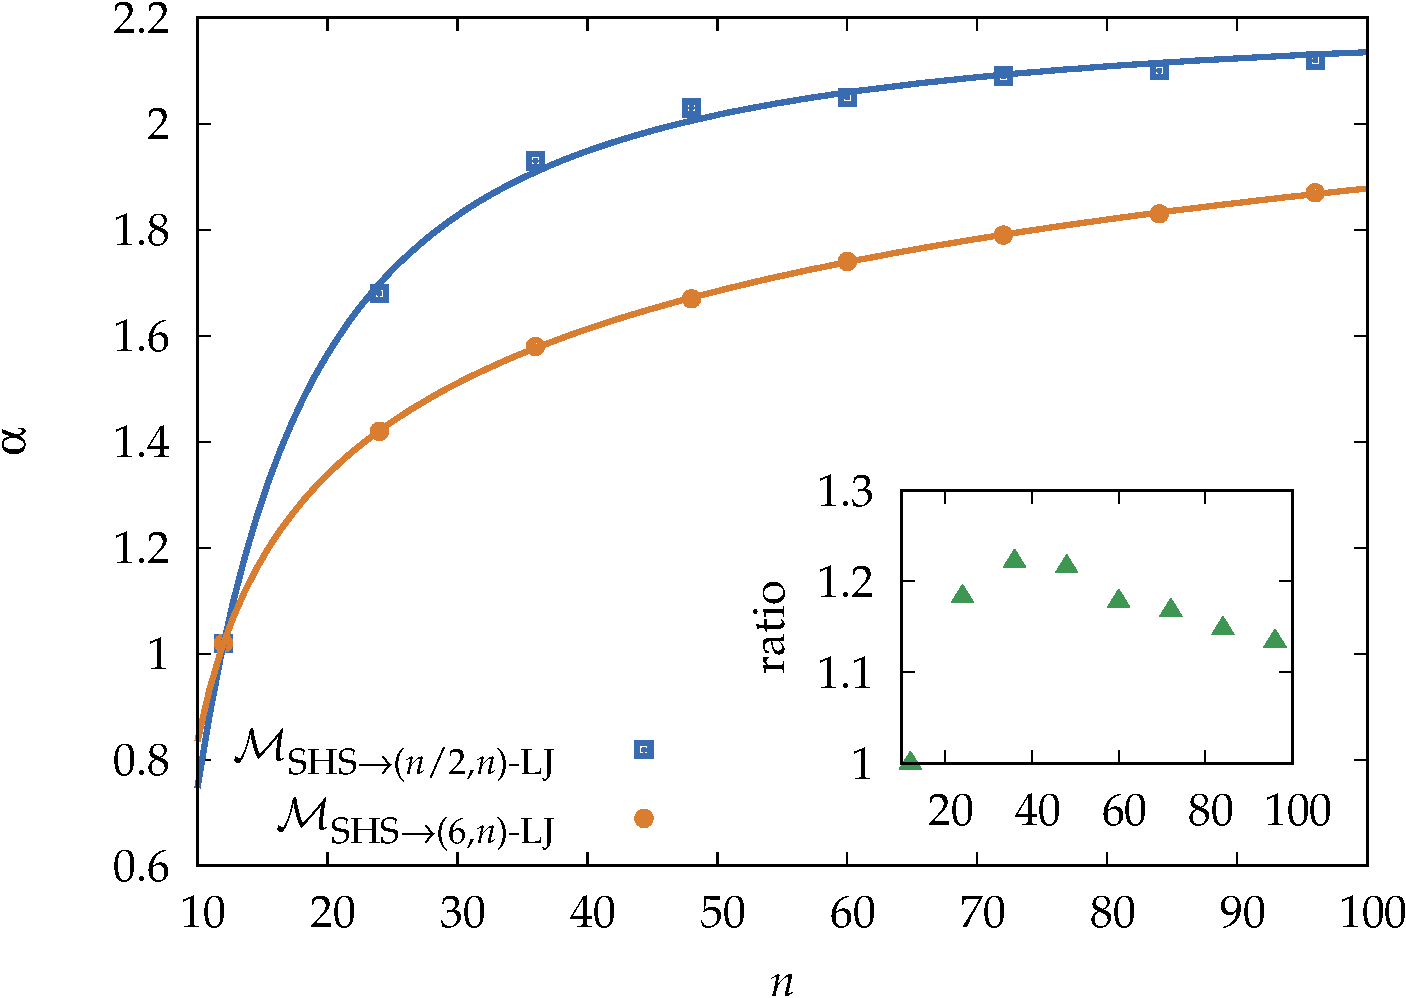
\includegraphics[width=0.8\columnwidth]{kslj/repulsive13-14.pdf}
	\caption{Convergence behaviour of the asymptotic exponential rise rate parameter
	$\alpha$ (Eq.(\ref{eq:Stil})) towards the SHS limit with respect to the LJ exponent $n$. The inlet shows the ratio of
	the two quantities $\alpha(|\mathcal{M}_{\text{SHS}\to (n/2,n)-\text{LJ}}(N)|) /
	\alpha(|\mathcal{M}_{\text{SHS}\to (6,n)-\text{LJ}}(N)|)$.}
    \label{fig:repulsive13-14}
\end{figure}


Using the results for $N \geq 13$ 
from Figure~\ref{fig:expinfty}, we can calculate how $\alpha$ depends on the LJ range parameter $n$.
As shown in Figure~\ref{fig:repulsive13-14}, a general function of the form
\begin{align}
\label{expgrowth}
    \alpha(n)=\alpha_\text{max}+\frac{a}{(n-n_0)^{p}}
\end{align}
fits the results nicely, allowing the prediction of growth behaviour for different
LJ potentials. For $|\mathcal{M}_{(n/2,n)-\text{LJ}}|$, $\alpha_\text{max}$ is
equivalent to $\alpha_\text{SHS}=2.207$. The other adjusted parameters are
$a=-66.588$, $n_0=-3.386$ and $p=1.473$ (Figure~\ref{fig:repulsive13-14}).
We also show the ratio $\alpha(|\mathcal{M}_{\text{SHS}\to (n/2,n)-\text{LJ}}|) /
	\alpha(|\mathcal{M}_{\text{SHS}\to (6,n)-\text{LJ}}|)$ between the two 
	different LJ asymptotic exponential rise rate parameters, which shows that larger
	cluster sizes need to be studied to correctly describe the asymptotic limit. 


The distribution of minima as a function of (free) energy was suggested to be
Gaussian \autocite{Sciortino-1999}.  Figure~\ref{fig:N13-steps} shows the energy
distribution of minima for different LJ $(n/2,n)$ potentials derived from SHS
initial structures. We do not see a Gaussian type of distribution; this 
result does not change if we take the free energy at finite temperatures. 
The results indicate a ``phase transition'' in the potential energy landscape away from low-energy to
high energy minima as $n$ increases.
The transition occurs at fairly small $n$. 
Results for the $(9,18)$-LJ potential indicate two HCR-SCA-like maxima that are not present for the $(6,12)$-LJ potential; these are associated with the $N_c = 34$ and $N_c = 35$ SHS clusters,
respectively.
It is also clear that (as expected) the distributions narrow with increasing $n$.

\begin{figure}
    \centering
    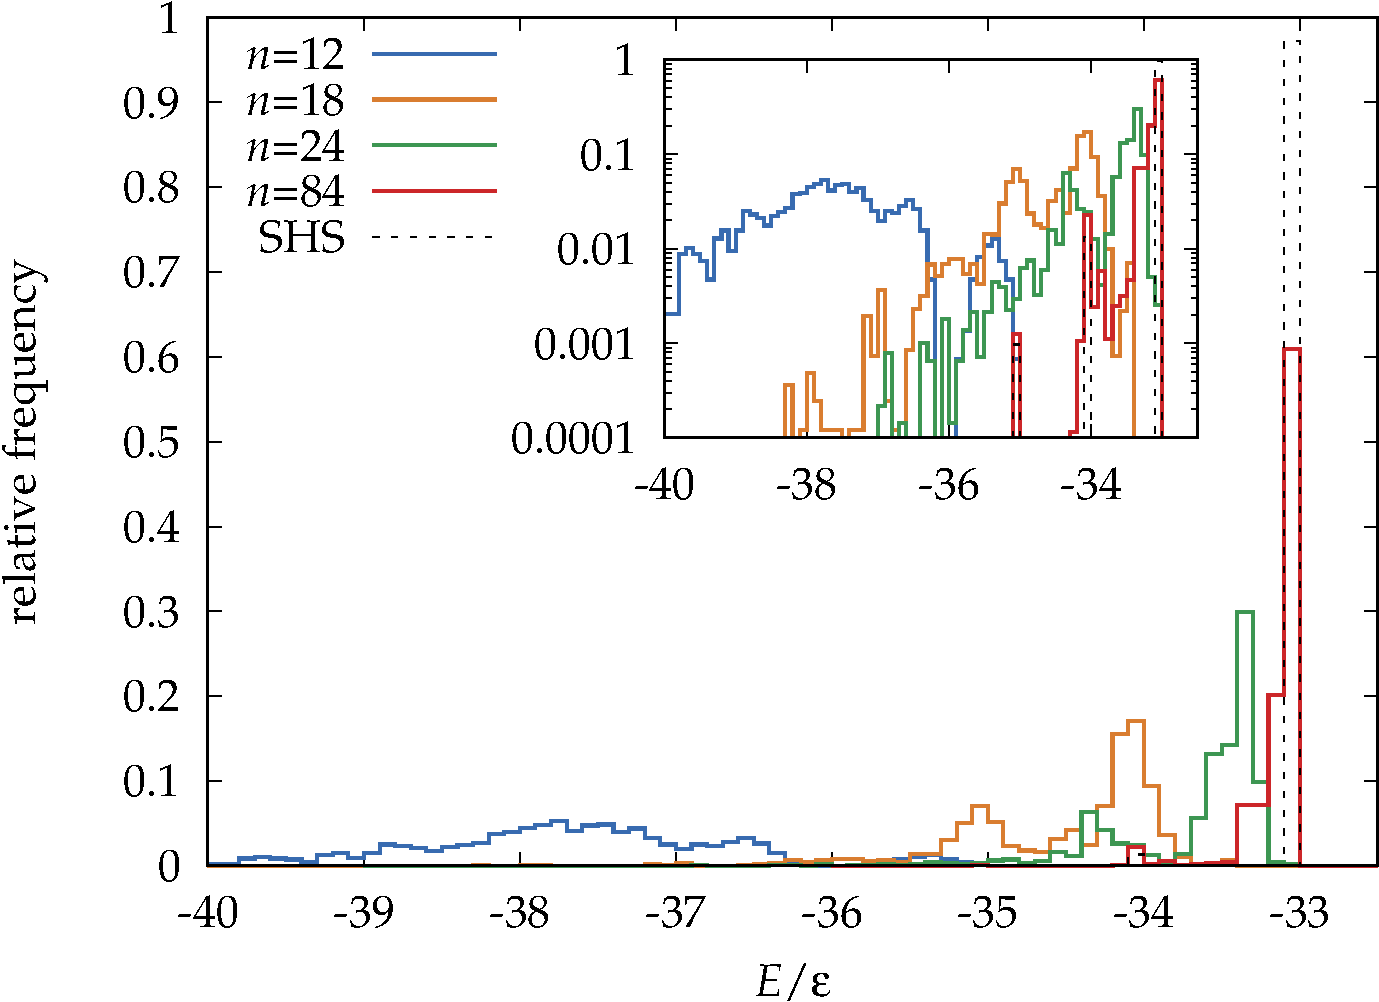
\includegraphics[width=0.8\columnwidth]{kslj/N13-steps.pdf}
    \caption{Histogram of the energies (bin size $\Delta\varepsilon=0.1$) of
    minima $\mathcal{M}_{\text{SHS}\to (n/2,n)-\text{LJ}}(N)$ for $N=13$ and
    different exponents $n$ up to the SHS limit. For better visibility, the
    height of the bars are set to $\Delta|\mathcal{M}|/|\mathcal{M}|$ in the
    interval $\Delta(E/\epsilon)$. The inlet shows the same data in logarithmic
    scale.}
    \label{fig:N13-steps}
\end{figure}



\begin{table}\centering
\resizebox{\linewidth}{!}{%
    \begin{threeparttable}
    \caption{Number of distinct local minima $|\mathcal{M}_\mathrm{SHS}|$ for
    cluster size $N$ (from Refs.~\cite{Holmes-Cerfon_EnumeratingRigidSphere_2016,Hoy_Structurefinitesphere_2012,Hoy_Structuredynamicsmodel_2015}) 
    and contact number $N_c$ from the exact enumeration, 
    compared to the number of different structures obtained from a
    geometry optimisation starting from the set $\mathcal{M}_{\mathrm{SHS\to
    LJ}}(N,N_c)$ for a (6,12)-LJ potential. The overall number of unique minima 
 $|\mathcal{M}_\mathrm{SHS\to LJ}|  = \sum_{N_c} |\mathcal{M}_\mathrm{SHS\to LJ} (N_c)| - (\# \mathrm{\ of\ duplicate\ structures})$    
 is shown in the following column. 
    This result can be compared to the number of unique minima found using the basin-hopping method
    ($|\mathcal{M}_\mathrm{LJ}|$). The difference $\Delta\mathcal{M}=|\mathcal{M}_\mathrm{LJ}| - |\mathcal{M}_\mathrm{SHS\to LJ}|$ 
    is also listed.}
    \label{tab:comp}
    \small{\begin{tabular}{clccccc}\toprule
        $N$ & $N_c$ & $|\mathcal{M}_\mathrm{SHS} (N_c)|$ & $|\mathcal{M}_{\mathrm{SHS\to LJ}}(N_c)|$ & $|\mathcal{M}_\mathrm{SHS\to LJ}|$ & $|\mathcal{M}_\mathrm{LJ}|$     &  $\Delta\mathcal{M}$ \\ \midrule
8  & 18  & 13     				& 8    & 8                     & 8                     & 0                   \\  \midrule
9  & 21  & 52     				& 20   & 20                    & 21                    & 1                   \\  \midrule
10 & 23  & 1      				& 1    &                       &                       &                     \\
   & 24  & 259    				& 60   & 62                    & 64                    & 2                   \\
   & 25  & 3      				& 3    &                       &                       &                     \\  \midrule
11 & 25  & 2      				& 2    & \multirow{6}{*}{165}  & \multirow{6}{*}{170}  & \multirow{6}{*}{5}  \\
   & 26  & 18     				& 6    &                       &                       &                     \\
        & 27  & 1620\tnote{a}	& 158  &                       &                       &                     \\
   & 28  & 20     				& 12   &                       &                       &                     \\
   & 29  & 1      				& 1    &                       &                       &                     \\  \midrule
12 & 28  & 11     				& 6    & \multirow{6}{*}{504}  & \multirow{6}{*}{515}  & \multirow{6}{*}{11} \\
   & 29  & 148    				& 24   &                       &                       &                     \\
   & 30  & 11638  				& 483  &                       &                       &                     \\
   & 31  & 174    				& 69   &                       &                       &                     \\
   & 32  & 8      				& 6    &                       &                       &                     \\
   & 33  & 1      				& 1    &                       &                       &                     \\  \midrule
13 & 31  & 87     				& 23   & \multirow{8}{*}{1476} & \multirow{8}{*}{1510} & \multirow{8}{*}{34} \\
   & 32  & 1221   				& 100  &                       &                       &                     \\
        & 33  & 95810\tnote{a}& 1418 &                       &                       &                     \\
        & 34  & 1318\tnote{a} & 293  &                       &                       &                     \\
   & 35  & 96     				& 49   &                       &                       &                     \\
   & 36  & 8      				& 6    &                       &                       &                     \\  \midrule
        14 & 33  & 1      				& 1    & \multirow{8}{*}{4093} & \multirow{8}{*}{(4187)\tnote{b}}    & \multirow{8}{*}{(94)\tnote{b}}  \\
   & 34  & 707    				& 101  &                       &                       &                     \\
   & 35  & 10537  				& 410  &                       &                       &                     \\
   & 36  & 872992 				& 3939 &                       &                       &                     \\
   & 37  & 10280  				& 1002 &                       &                       &                     \\
   & 38  & 878    				& 237  &                       &                       &                     \\
   & 39  & 79     				& 42   &                       &                       &                     \\
   & 40  & 4      				& 3    &                       &                       &                     \\\bottomrule
    \end{tabular}}
        \begin{tablenotes}
        \item[a]{The largest value for $|\mathcal{M}_\mathrm{SHS}|$ has been taken from 
    Refs.~\cite{Holmes-Cerfon_EnumeratingRigidSphere_2016,Hoy_Structurefinitesphere_2012,Hoy_Structuredynamicsmodel_2015}.}
        \item[b]{Estimated.}
        \end{tablenotes}
    \end{threeparttable}}
\end{table}%


It is well known that the global minimum for rare gas clusters with 13 atoms is
the ideal Mackay icosahedron \autocite{Hoare_Physicalclustermechanics_1975,Hoare_Statisticalmechanicsmorphology_1976,Hoare_StructureDynamicsSimple_2007}. Simple
geometric considerations imply that such a symmetric cluster is not possible
for sticky hard spheres; all vertices of a regular icosahedron with unit edge length
lie on a circumscribing sphere with radius $r_c\approx 0.951$, making it
impossible to insert a sphere of the same radius into the center of the
polyhedron.  Therefore, there must be well-defined LJ exponents $(m,n)$ at
which the icosahedral $N = 13$ LJ cluster breaks symmetry to form a rigid cluster.  
For the $n = 2m$ case considered above, this symmetry-breaking occurs at $m \simeq 15$.

We also explored a more realistic extended LJ potential (Eq.\ \ref{eq:ELJ};  Figure~\ref{fig:LJ})
for one of the rare gas dimers (xenon) 
in comparison with other LJ potentials. We see that the repulsive part agrees
nicely with the conventional (6,12)-LJ potential, while for $r > 1$
the extended LJ potential is slightly less attractive. 
This change should lead to an increase in the number of local minima compared to the conventional
(6,12)-LJ potential. We find that this is indeed the case, i.e.
$|\mathcal{M}_\mathrm{SHS\to ELJ}|=\{8,21,74,205,685,2179,6863\}$ for
$N=\{8,9,10,11,12,13,14\}$.  For $N=13$ the number of distinct minima is 44\% larger than it is for the simple (6,12)-LJ potential,
which shows that $|\mathcal{M}(N)|$ is rather sensitive to the potential chosen.
Hence, to correctly describe the topology of real systems, one has to take care
of the correct form of the 2-body contribution (as well as higher $n$-body
contributions) \autocite{Schwerdtfeger-2016}.



%\subsection{(6,12)-Lennard-Jones cluster from basin-hopping}
\subsection{(6,12)-Lennard-Jones clusters from basin-hopping} 

Table~\ref{tab:comp} shows the number of distinct minima found by our cluster
geometry optimisation procedure using the (6,12)-LJ potential compared to
results from exact enumeration for SHSs and from basin-hopping for the (6,12)-LJ
potential.  As the SHS clusters for a specific $N$ value can be grouped by
their contact number $N_c$, the geometry optimisations were carried out
separately for each group of $\mathcal{M}_\mathrm{SHS}(N_c)$. Hoy
\autocite{Hoy_Structurefinitesphere_2012,Hoy_Structuredynamicsmodel_2015} and Holmes-Cerfon~\autocite{Holmes-Cerfon_EnumeratingRigidSphere_2016}  reported
slightly different results
for $N=11$ and $N=13$; we find that upon geometry optimisation,
their datasets yield the same final clusters
$|\mathcal{M}_{\mathrm{SHS\to LJ}}(N_c)|$.  As identical LJ clusters appear in
multiple groups with different contact numbers, we remove the duplicates to
create the set $\mathcal{M}_\mathrm{SHS\to LJ}$ of distinct minima, which can
be directly compared to the set of LJ minima $\mathcal{M}_\mathrm{LJ}$ obtained
from the basin-hopping method. It should be noted that including the hypostatic
clusters and the different $|\mathcal{M}_\mathrm{SHS}|$ for $N=11$ and $N=13$
from Ref.~\autocite{Holmes-Cerfon_EnumeratingRigidSphere_2016} did not change our results, implying that hypostatic
clusters are not an important feature for the LJ energy landscape. 


Interestingly, our gradient-based minimisation procedure starting from the SHS
packings does not in general lead to a complete set of LJ minima; the mapping
from SHS minima to LJ minima is non-injective and non-surjective.  Clearly,
some structural motifs found in LJ clusters are not found in SHS clusters and
vice versa, and the topology of the hypersurface changes in a non-trivial
fashion from SHS to LJ.  However, it is surprising that the fraction of
structures that are missed by this optimisation procedure is so small (see
Table~\ref{tab:seeds}). To gain further insight, we analysed the energetics and
structure of the unmatched clusters in more detail.

%
%
\begin{table}\centering
    \begin{threeparttable}
    \caption{Number of missing structures after optimisation belonging to the
    same "seed" (Fig.\ \ref{fig:seeds}). $N=8$ is excluded because all LJ minima were
    found starting from the SHS model.}
    \label{tab:seeds}
    \begin{tabular}{llllll}\toprule
        seed      & $N=9$   & $N=10$  & $N=11$  & $N=12$  & $N=13$  \\ \midrule
        a         & 1    & 1    & -    & 3    & 8    \\
        b         & -    & 1    & 3    & 4    & 12\tnote{a}   \\
        c         & -    & -    & 1    & 1\tnote{a}    & -    \\
        d         & -    & -    & 1    & 1    & 5    \\
        e         & -    & -    & -    & 1    & 6    \\
        f         & -    & -    & -    & 1    & 1    \\
        remaining & -    & -    & -    & -    & 2    \\ 
        total     & 1    & 2    & 5    & 11   & 34   \\
        \%        & 4.76 & 3.13 & 2.94 & 2.14 & 2.25 \\ \bottomrule
    \end{tabular}
        \begin{tablenotes}
        \item[a]{Some structures do not resemble a perfect capped
        cluster, but undergo a slight rearrangement. Specifically, two structures belonging to seed (b) and one structure belonging to seed (c) were found to deviate slightly from the perfect arrangement, but minor rearrangements of these structures lead to the desired geometry and they can be reasonably associated with these seeds.}
        \end{tablenotes}
    \end{threeparttable}
\end{table}%
%
%
\begin{figure}
    \centering
    \subfloat[$N=11$]{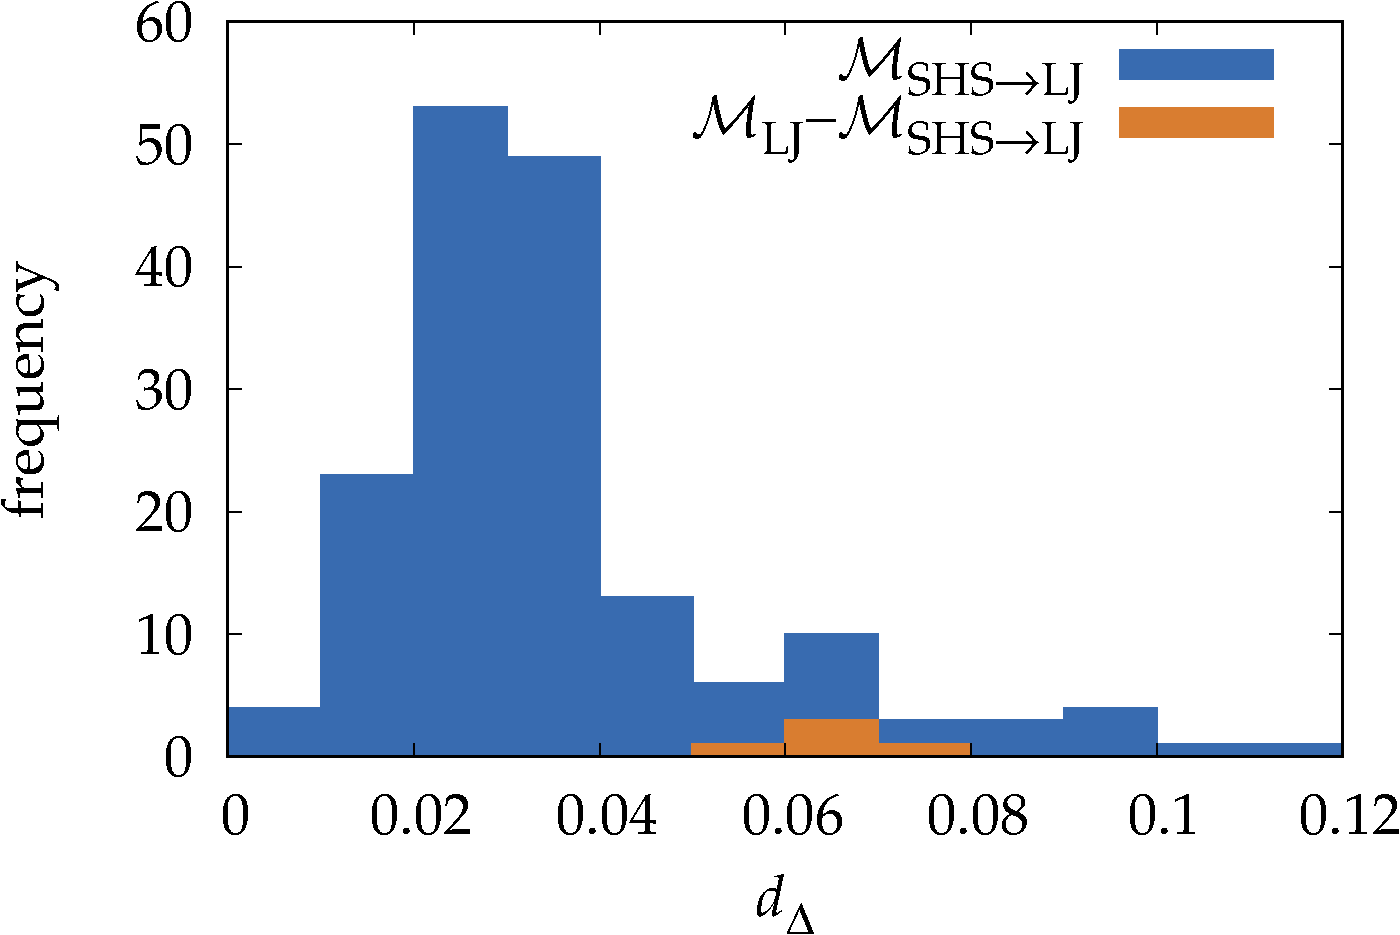
\includegraphics[width=.5\textwidth]{kslj/lj11var.pdf}}
    \subfloat[$N=12$]{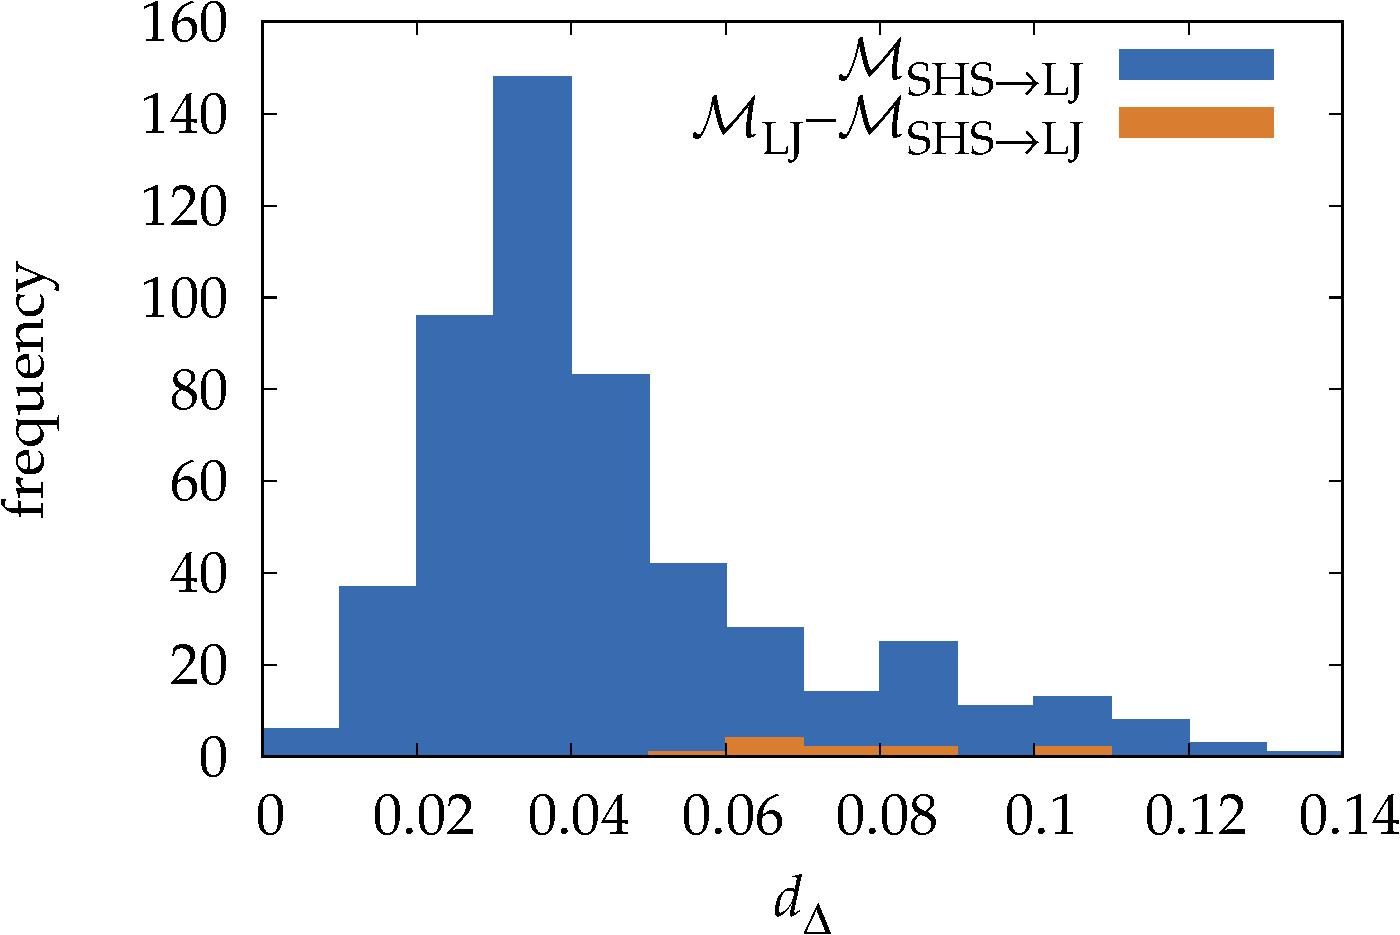
\includegraphics[width=.5\textwidth]{kslj/lj12var.pdf}}\\
    \subfloat[$N=13$]{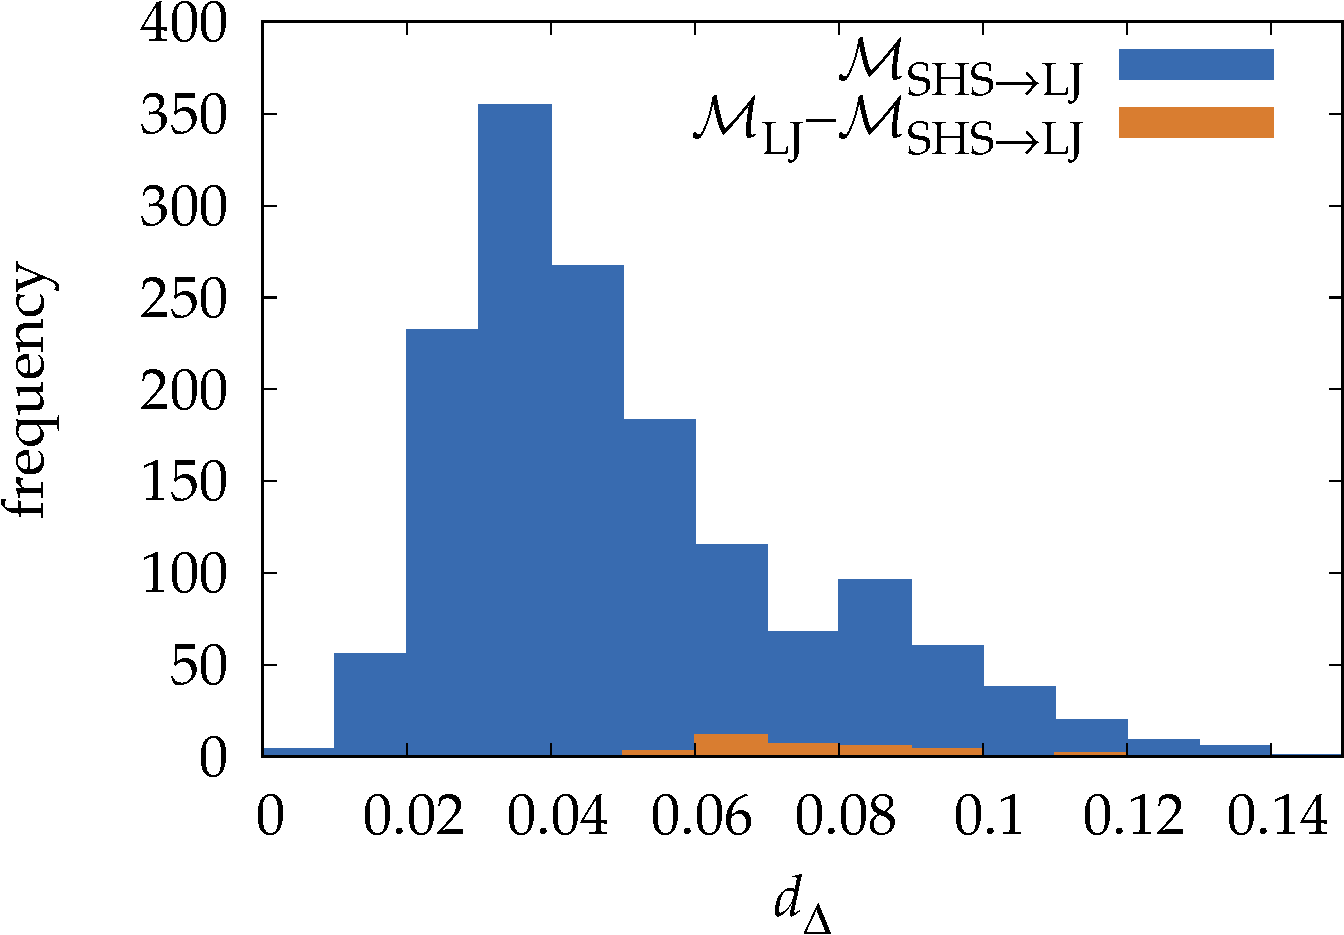
\includegraphics[width=.5\textwidth]{kslj/lj13var.pdf}}
    \caption{Histograms of the difference between the longest and shortest bond
    distances $d_\Delta=d_\text{max}-d_\text{min}$ for the complete set of
    distinct LJ minima $\mathcal{M}_\text{LJ}(N)$ for $N=\{11,12,13\}$. Orange
    bars give the number of distinct structures not contained in
    $\mathcal{M}_\mathrm{LJ}$ as obtained from the basin-hopping algorithm.}
    \label{fig:bondlength-variance}
\end{figure}%
%
%
Figure~\ref{fig:bondlength-variance} shows an analysis of the difference
between the longest to the shortest bond lengths $d_\Delta=d_{\mathrm max}-d_{\mathrm
min}$ obtained for the largest clusters in $\mathcal{M}_{\mathrm{LJ}}$ with
$N=\{11,12,13\}$ \footnote{We define spheres that have a equilibrium distance
between $0.9-1.1$ to be bound.}.  The histograms show that the clusters most
commonly have a $d_\Delta$ of about $0.03$.  In contrast, as shown by the
orange bars, the unmatched structures have significantly larger $d_\Delta$
values of at least $0.05$, with most of them having $d_{\Delta} \simeq 0.06$.
This is a first indication of why these structures are not found by starting
from SHS packings. The latter only form bonds of length one, and a large
variation in bond length could imply that a SHS packing similar to the LJ
structure does not exist as the SHS boundary conditions are not satisfied.  The
data in Table~\ref{tab:energies} show that the unmatched (UM) structures for a
specific $N$ value have much higher energies compared to the one of the global
minimum (which is set to zero, i.e.  $E_0=0$). % 
%
\begin{table}\centering
    \caption{Range $[E_0,E_\text{max}]$ of the energy spectrum of all LJ
    minima, position of the second lowest minimum structure $E_1$ and position
    of the first unmatched (UM) structure $E_0^\text{UM}$ relative to the
    respective global minimum (in reduced units and $E_0=0$).}
    \label{tab:energies}
        \begin{tabular}{lccc}\toprule
        $N$ & $E_\text{max}$ & $E_1$ & $E_0^\text{UM}$ \\\midrule
        8   & 1.04   & 0.06    & -           \\
        9   & 2.08   & 0.84    & 1.19        \\
        10  & 3.13   & 0.87    & 2.22        \\
        11  & 4.22   & 0.85    & 2.27        \\
        12  & 6.16   & 1.62    & 3.38        \\
        13  & 9.26   & 2.85    & 6.14        \\\bottomrule
        \end{tabular}
\end{table}%
%
They are always positioned in the upper half of the energy spectrum, making
them energetically unfavorable.  However, we could not find any correlation
between $d_\Delta$ and the energetic position of the LJ clusters.

\begin{figure}
    \centering
    \subfloat[]{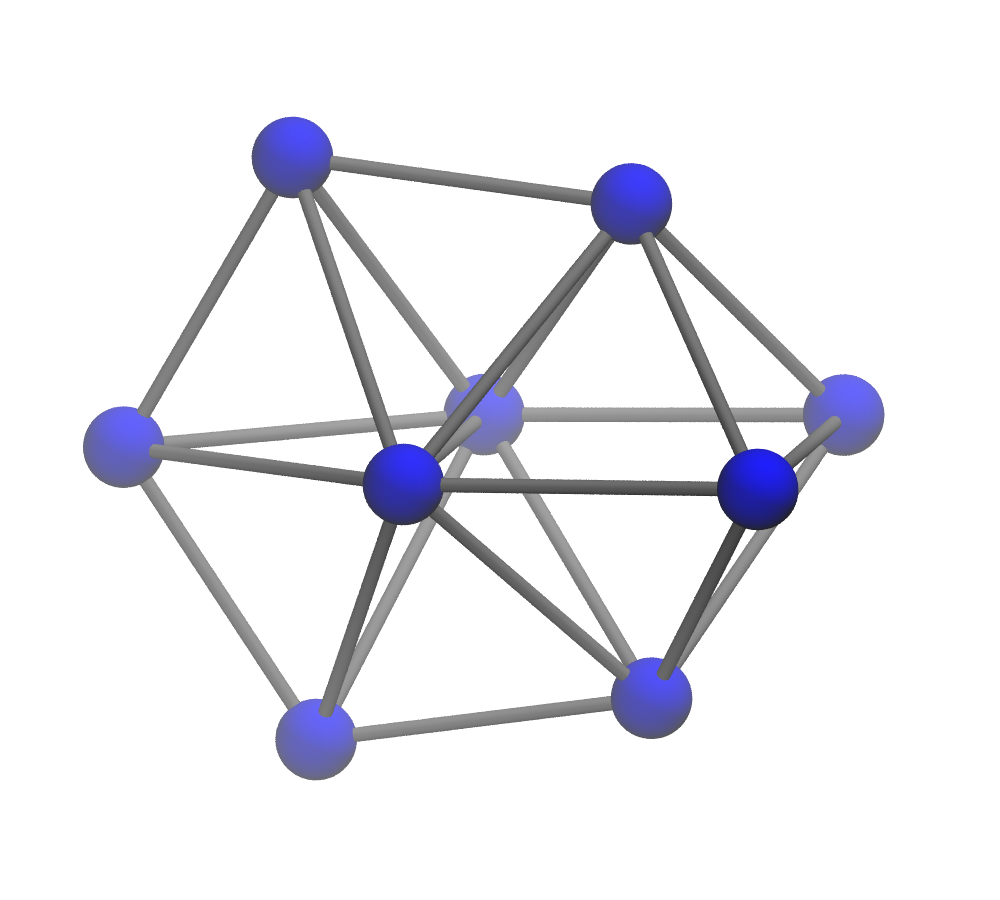
\includegraphics[width=0.26\columnwidth]{kslj/A.png}}
    \subfloat[]{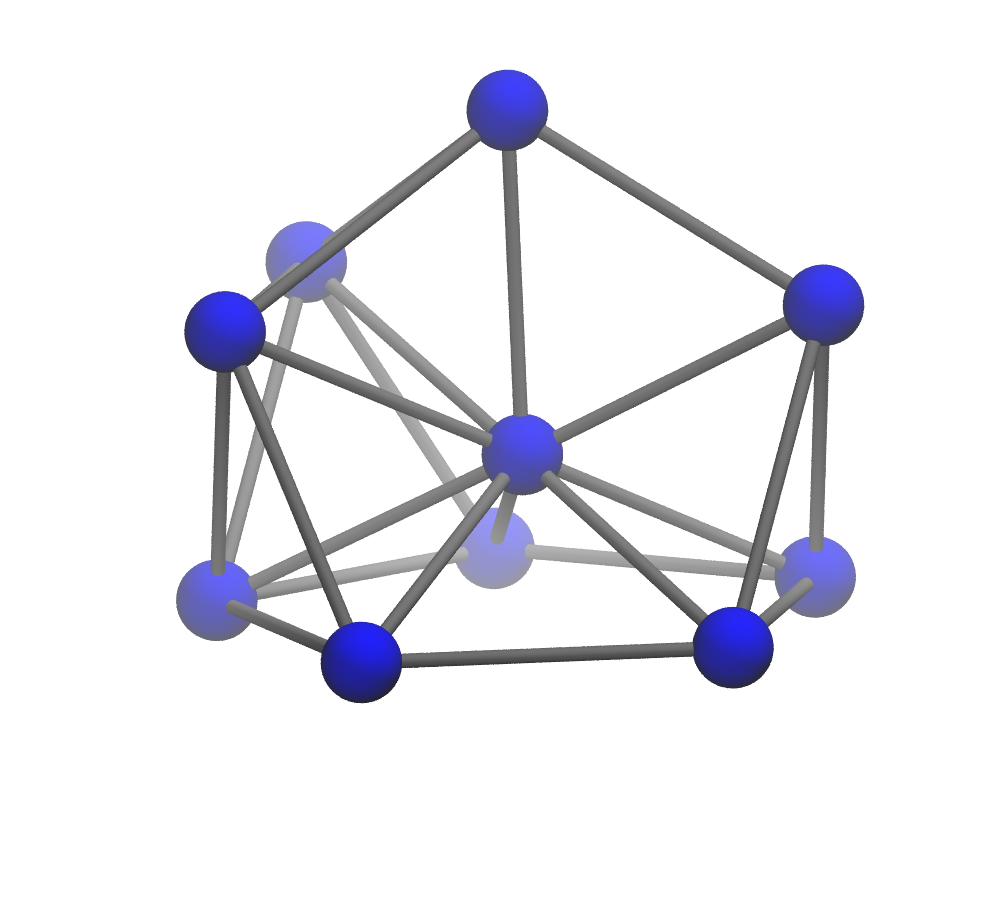
\includegraphics[width=0.26\columnwidth]{kslj/B.png}}
    \subfloat[]{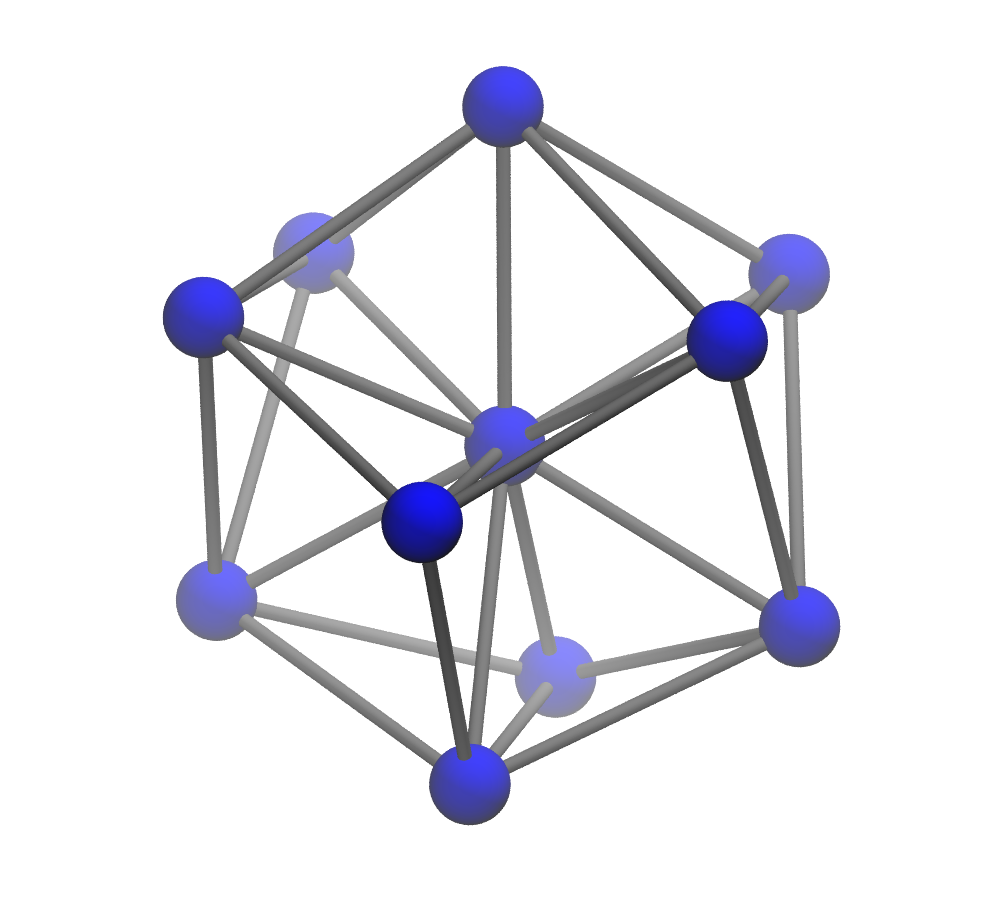
\includegraphics[width=0.26\columnwidth]{kslj/C.png}}\\
    \subfloat[]{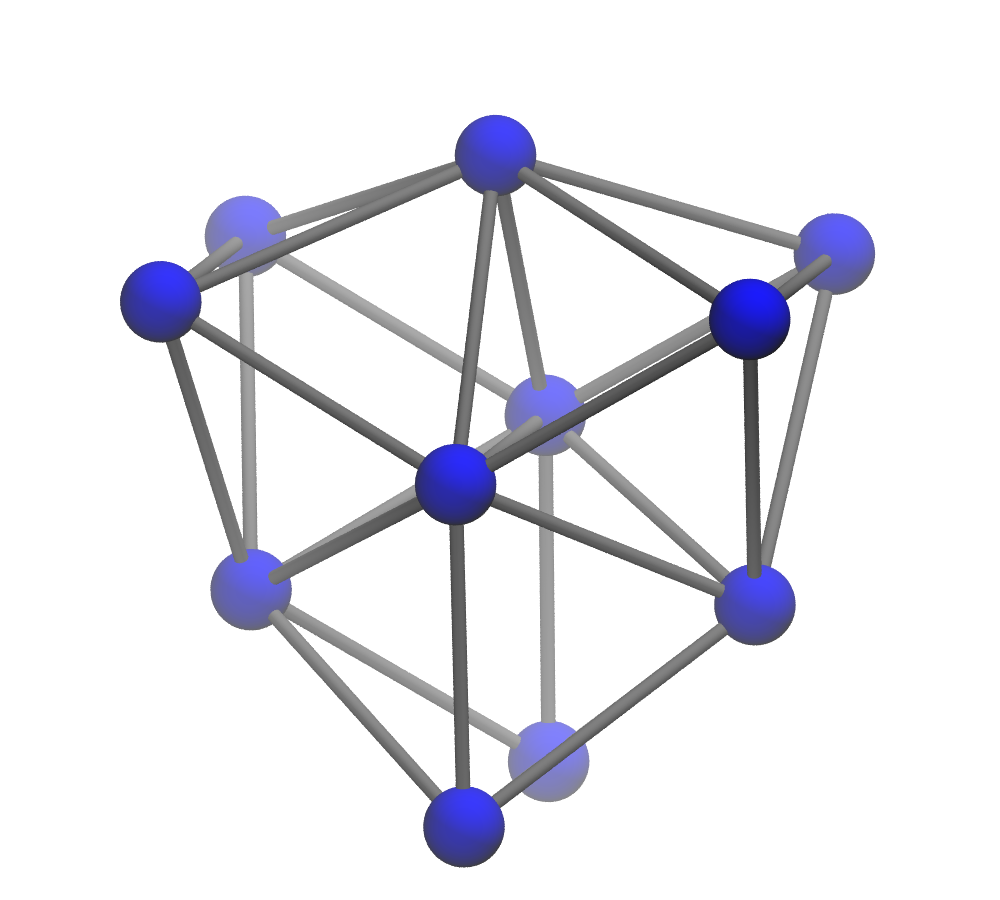
\includegraphics[width=0.26\columnwidth]{kslj/D.png}}
    \subfloat[]{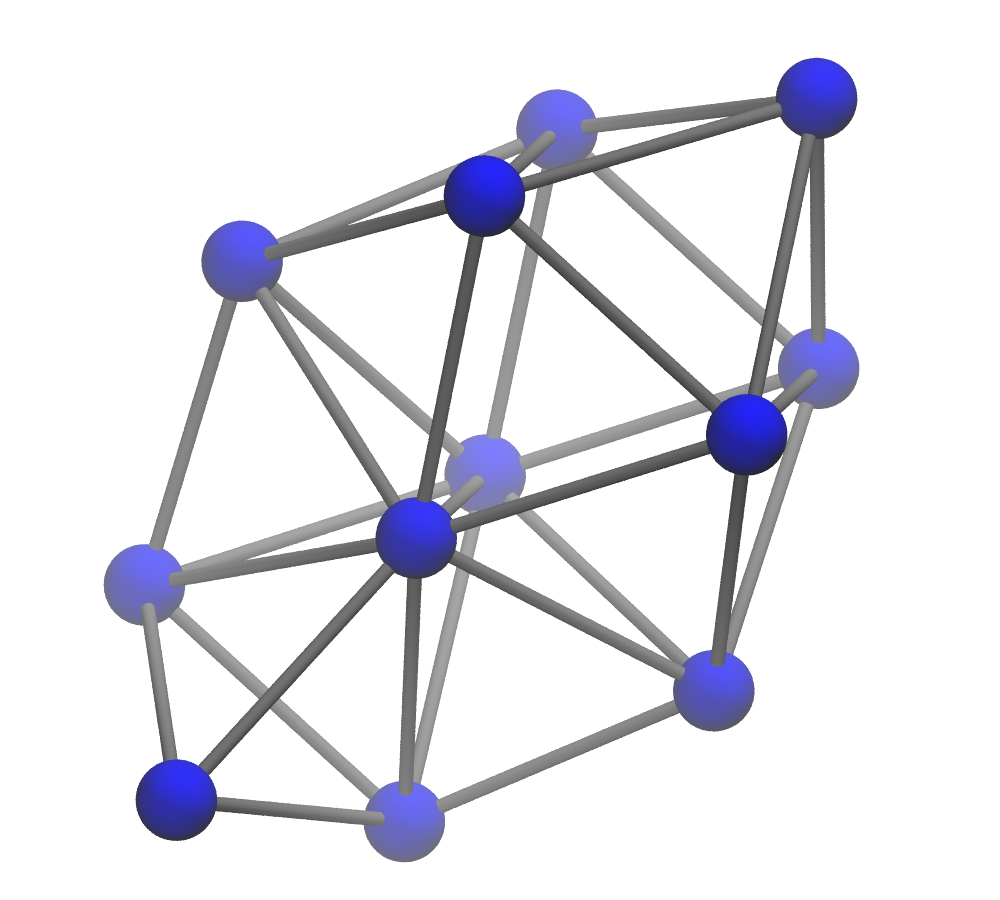
\includegraphics[width=0.26\columnwidth]{kslj/E.png}}
    \subfloat[]{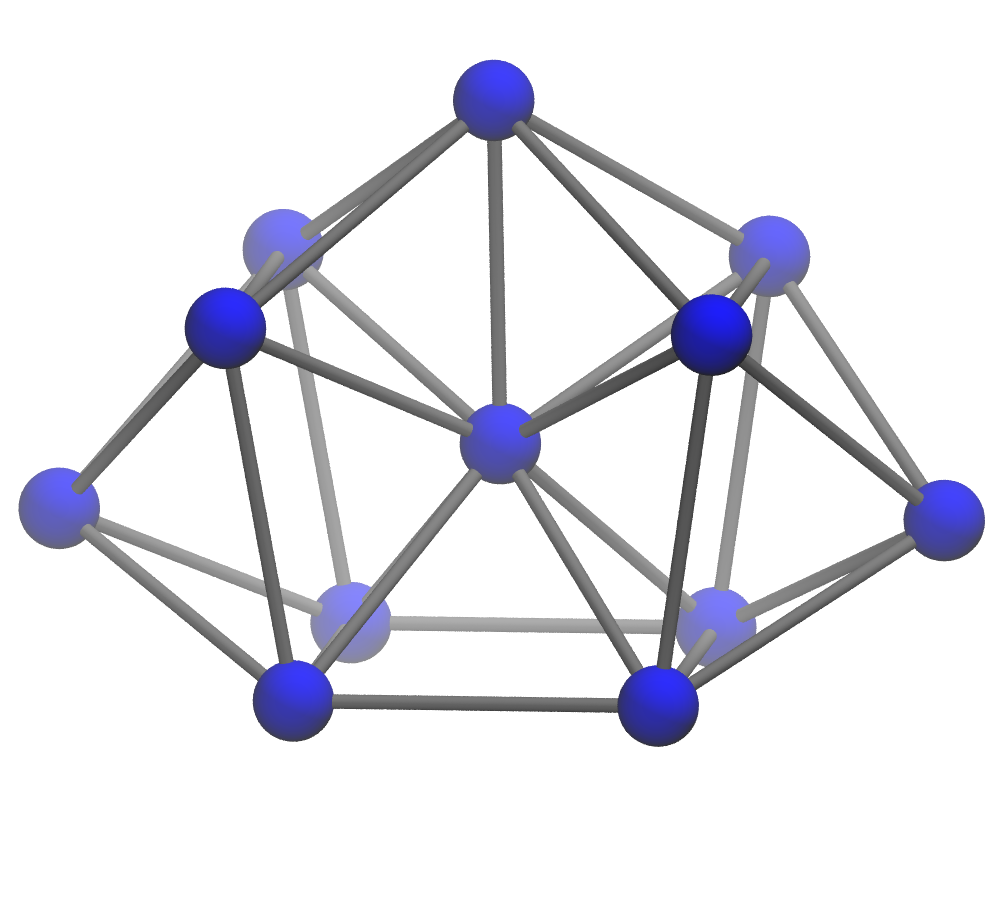
\includegraphics[width=0.26\columnwidth]{kslj/F.png}}
    \caption{Graphical representations of the structures that are starting new
    seeds, but are not contained in $\mathcal{M}_\mathrm{SHS\to LJ}$. See
    Table~\ref{tab:seeds} and text for more details.}
    \label{fig:seeds}
\end{figure}%

Last, we checked the geometries of the missing structures in more detail.
As it turns out, almost all of the missing stable LJ clusters can be created
from a smaller set of missing clusters by capping some of their triangular
faces. Therefore, these groups of clusters can be referred to as ``seeds''
\autocite{Arkus_DerivingFiniteSphere_2011}. The corresponding starting structures of each seed
are shown in Figure~\ref{fig:seeds}. 
None of these structures are stable SHS packings. For
example, structure (d) can be described as three octahedra connected via
triangular faces sharing one edge. Geometric considerations \autocite{Arkus_DerivingFiniteSphere_2011,Hoy_Structurefinitesphere_2012} immediately show
that this structure cannot be a stable SHS packing;
the dihedral angle in an octahedron is approximately $109.5^\circ$, which means three
octahedra only fill $328.5^\circ$ of a full circle, leaving a gap between two
faces. 


Table~\ref{tab:seeds} shows the number of missing minima belonging to each seed.
Over 60~\% of the unmatched structures belong to seeds (a) and (b).  
From a graph theoretical point of view \autocite{Arkus_Minimalenergyclusters_2009,Arkus_DerivingFiniteSphere_2011},
grouping structures into seeds means that all structures belonging to the same
seed contain the graph of the starting structures as a subgraph in their
respective connectivity matrix.  This approach simplifies the analysis to a
great extent, as the feature that prevents the structures from being found by
geometry optimisation is the same for each of the structures arising from a
specific seed.  
The smallest unmatched structures that cannot be associated with any of seeds (a)-(f) have $N=13$;
these could be the starting structures for two new seeds.


Finally, we note that the starting SHS minima in our optimisation procedure are
not stationary points on the LJ hypersurface, and we therefore optimise to most
but not all local and available LJ minima. This observation explains why some high-energy
structures were not found by our optimisation procedure. For a smooth change in the topology of the potential energy surface
from SHS to LJ type clusters one has to continuously vary the exponents $(m,n)$
in real space, which is computationally too demanding.


\chapter[The Gregory-Newton Clusters]{
    The Gregory-Newton Clusters\footnote{This chapter is partly composed of sections
    previously published in the article ``From Sticky-Hard-sphere to
    Lennard-Jones-Type Clusters''\autocite{} and is reproduced with kind
    permission from the authors and APS (\textcopyright 2018 American Physical
    Society).}
}
\label{sec:thegregorynewtonclusters}

\section{Introduction}
\label{sec:introductiongregorynewton}

\section{Results}
\label{sec:resultsgregorynewton}

\subsection{The Gregory-Newton Problem for Soft Potentials}
\label{sec:thegregorynewtonproblemforsoftpotentials}

The question of the Newton number in three dimensions has been resolved almost
70 years ago\autocite{Schutte_ProblemdreizehnKugeln_1952}. The proof is valid for hard-sphere
short-range potentials, but little is known about the behaviour of such
clusters under long-range potentials such as the Kratzer
potential\autocite{Kratzer_ultrarotenRotationsspektrenHalogenwasserstoffe_1920}. We used the optimisation
procedures explained in chapter~\ref{sec:theprogramspheres} to minimise the
energy of a starting structure consisting of 13 spheres surrounding a center
sphere with a fixed distance of one. Generating such a starting structure where
all surrounding spheres are evenly spaced is impossible since there exists no
triangulation of a sphere with 13 vertices, where every vertex has degree five
or six\autocite{Schwerdtfeger_topologyfullerenes_2015}. To generate an approximate
distribution we used the Fibonacci sphere
algorithm\autocite{Gonzalez_MeasurementAreasSphere_2010,Keinert_SphericalFibonacciMapping_2015} and used
this structure as a starting point for optimisations with \ac{LJ} potentials
with small exponents. The difference between the largest and smallest \ac{COS}
distance was used as a measure for whether the 13th sphere enters the first
coordination shell. A value of zero would be expected for this to be true.

\begin{figure}
    \centering
    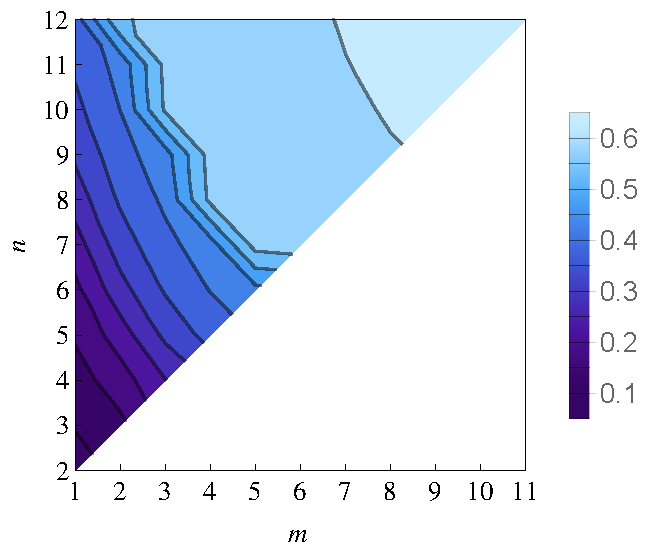
\includegraphics[width=.8\textwidth]{gregory-newton/N14.pdf}
    \caption{Relation of LJ exponents m and n to the difference of largest and
    smallest \ac{COS} distances.  A value of zero would imply that all
    surrounding spheres are touching the center sphere.}
    \label{fig:gregorynewton-N14}
\end{figure}

The results for all positive integer combinations of $m\leq11$ and $n\leq12$
with $m<n$ are depicted in figure~\ref{fig:gregorynewton-N14}. Even for the
combination of smallest exponents (1,2)-\ac{LJ} it is clear that the \ac{COS}
distances vary from sphere to sphere. For this potential the largest \ac{COS}
distance is $r_\text{max}=0.882$, while the shortest one is
$r_\text{min}=0.804$. While the longest distance only shows up once, the
shortest distance appears twice. All other 10 distances fall in the range
between $r = 0.845$ and $r = 0.861$. The $r_\text{max} /r_\text{min}$ ratio is
$1.097$ and much shorter compared to $r_\text{max} /r_\text{min}= \sqrt{2}$ for
the closed packed lattice, or the shortest distance possible for the \ac{SHS}
system which is $r_{14}^\text{GN} = 1.347$ (see discussion below). Hence the
13th sphere ``almost'' touches the center sphere.

Note that all \ac{COS} distances for the $N=14$ (1,2)-\ac{LJ} cluster are
significantly shorter than $r=1$, due to the $N(N-1)/2$ attractive two-body
interactions and the softness of the potential.  For infinite (e.g.
body-centered cubic or close-packed) lattices of particles interacting via
$V^\mathrm{LJ}_{mn}(r)$ with $n> m >3$, one can prove
\autocite{Schwerdtfeger_ExtensionLennardJonespotential_2006} that the nearest neighbor distance is
%
\begin{equation}
    r_\mathrm{NN}(m,n)=\left( L_n L_m^{-1}\right)^\frac{1}{n-m}. %{\color{red} < 1.}
    \label{eqn:lattice}
\end{equation}%
%
Here $L_n$ is the Lennard-Jones-Ingham lattice coefficient for a specific
lattice determined from 3D lattice sums.  Since $L_n<L_m$ for $n>m$, we see
that $r_\mathrm{NN}<1$, and $\lim\limits_{m,n\rightarrow
\infty}r_\mathrm{NN}(m,n)=1$.  The shortest distances found in (6,12)-\ac{LJ}
clusters $r_\text{min}(N)$ are: $r_\text{min}(8)=0.986767$,
$r_\text{min}(9)=0.964404$, $r_\text{min}(10)=0.964382$,
$r_\text{min}(11)=0.956345$, $r_\text{min}(12)=0.947842$, and
$r_\text{min}(13)=0.952179$.  Surprisingly, $r_\text{min}(12)$ is smaller than
$r_\mathrm{NN}(6,12)$ for typical crystalline lattices; $r_\mathrm{NN}(6,12)$
values are $0.95066$, $0.95186$ and $0.97123$ for simple cubic, body-centered
cubic and close-packed lattices, respectively.  This result shows that stable
clusters do not necessarily have longer bonds compared to the solid state,
where we expect a maximum in interaction energy per atom.


\subsection{The Smallest Gregory-Newton Clusters}
\label{sec:themsmallestgregorynewtonclusters}

Ref.~\cite{Holmes-Cerfon_EnumeratingRigidSphere_2016} contains a putatively
complete set of hard-sphere clusters with $N=13$ and $N=14$.  We find a
surprisingly large number ($737$) of nonisomorphic $N = 13$ \ac{GN}-\ac{SHS}
structures ($\{724,10,1,2\}$ for $N_c=\{33,34,35,36\}$), that all optimise to
the ideal icosahedral arrangement ($I_h$ symmetry) if a $(6,12)$-\ac{LJ}
potential is applied. This large number results from the fact, that the 12
spheres surrounding the center sphere can't be arranged with icosahedral
symmetry. Since all of these structures seem to be related to the icosahedron
by geometry optimisation we investigated their shell structures
graph-theoretically. We define the shell to be the polyhedron created by the 12
spheres surrounding the center sphere. The graphs of the shells can now be
compared to the ideal icosahedral graph depicted in figure~\ref{fig:icograph}.

\begin{figure}
    \centering
    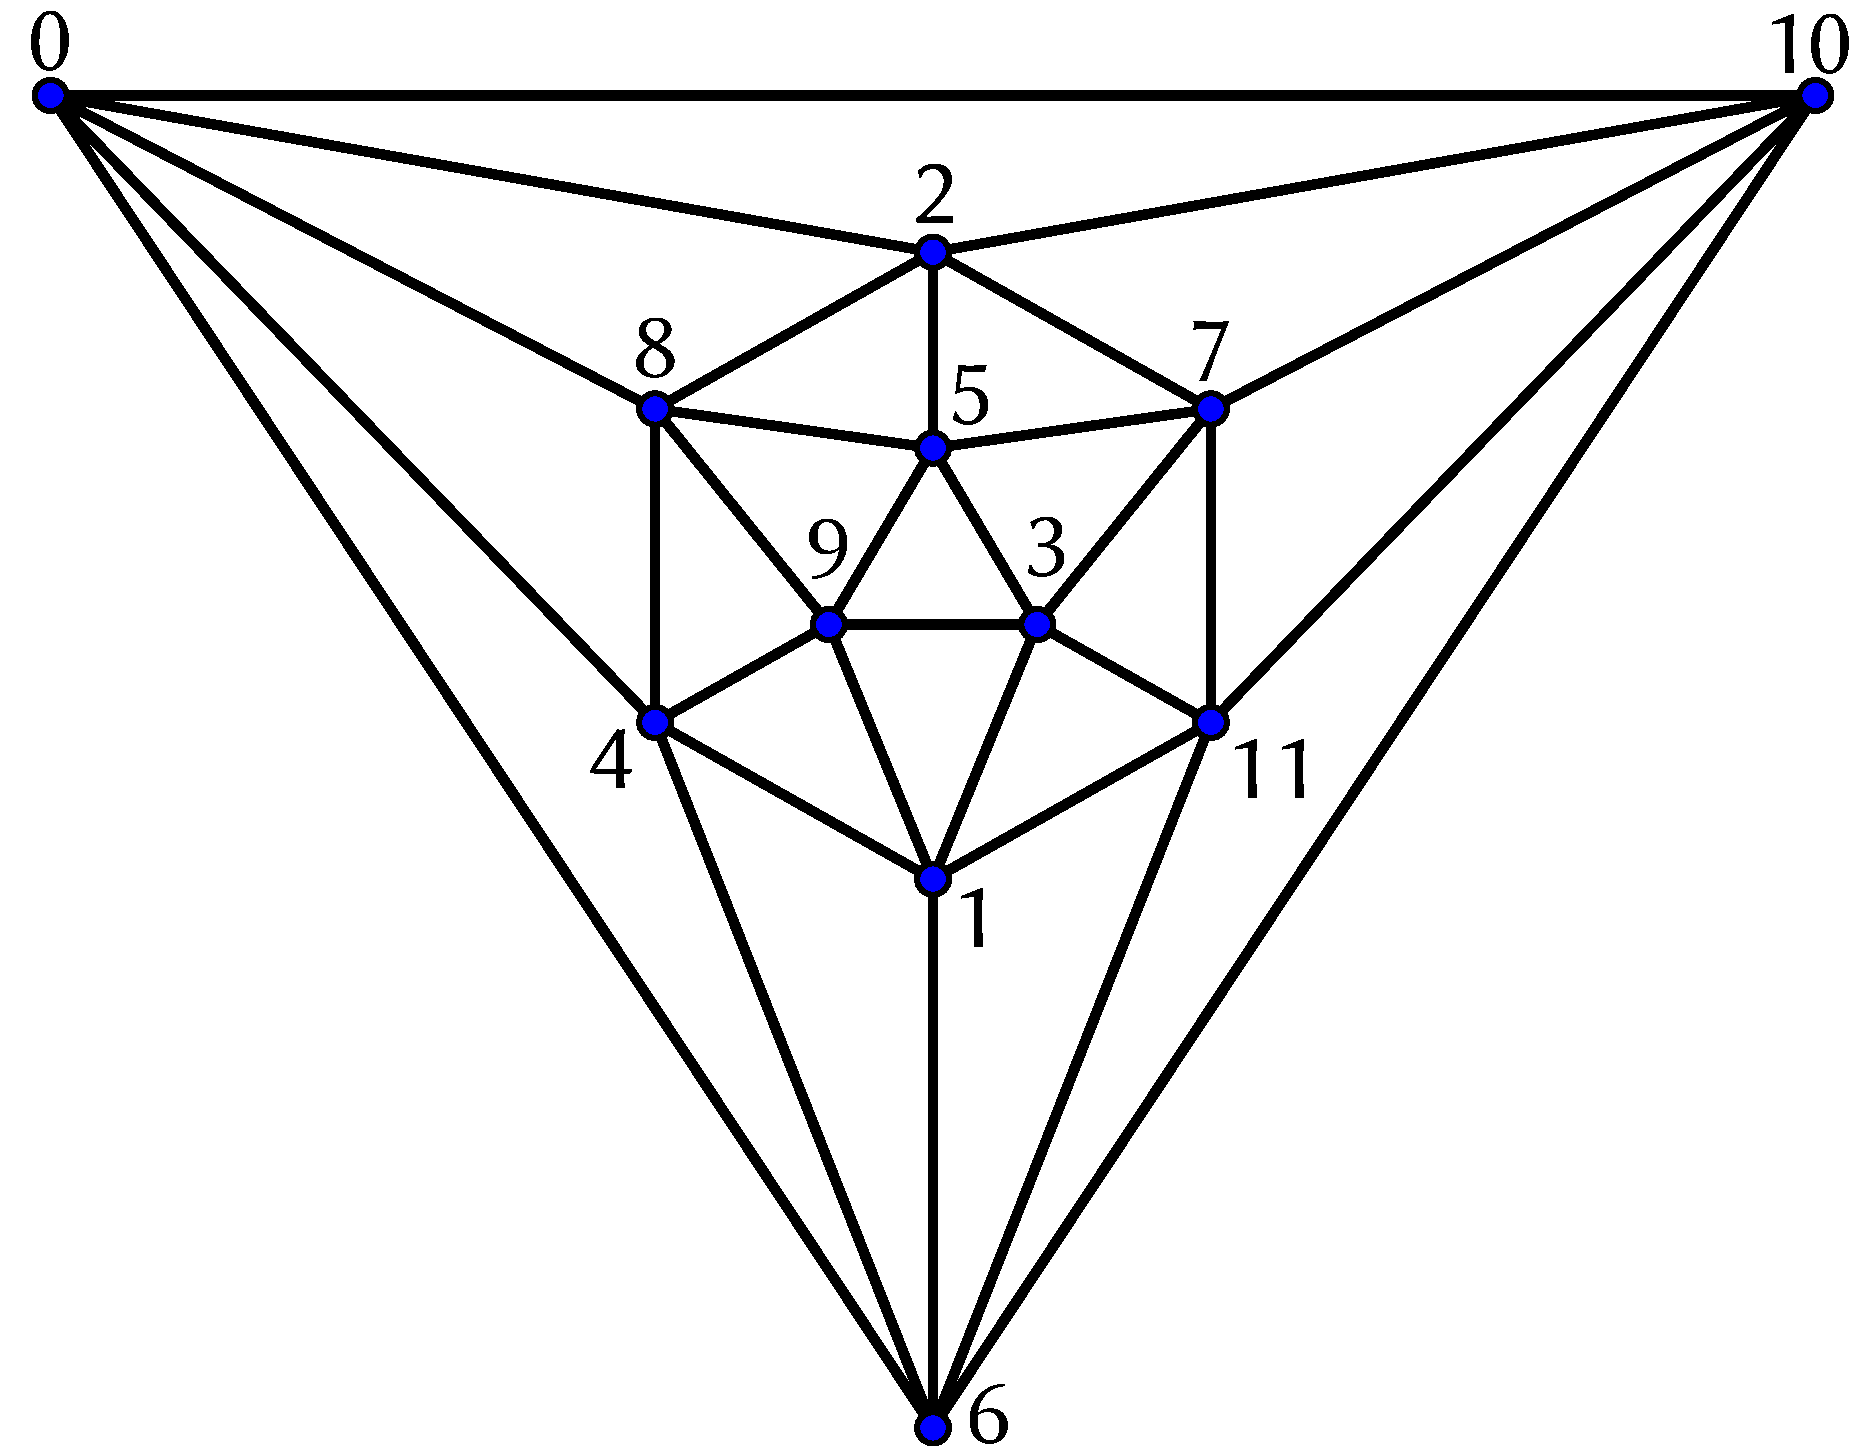
\includegraphics[width=.8\textwidth]{gregory-newton/ico.pdf}
    \caption{Two-dimensional projection of the icosahedral graph. Numbers refer
    to the respective node index.}
    \label{fig:icograph}
\end{figure}

We used the \textit{VF2} algorithm\autocite{Cordella_SubGraphIsomorphism_2004}
as implemented in the \textit{boost} graph library\autocite{_boost_2002} to
check the graphs of the \ac{GN} shells for subgraph-isomorphism with respect to
the icosahedral graph. Including edge-induced subgraphs we find all 737
12-sphere shells to be subgraphs of the icosahedral graph, which means their
vertices can all be mapped to vertices of the icosahedral graph such that there
will be no edges not present in the icosahedral graph. The graphs of the
12-sphere shells can now be described in terms of removed edges with respect to
the icosahedral graph. An extensive list of all subgraphs is included in
appendix~\ref{sec:listofgregorynewtonshells} (table~\ref{tab:icosubgraphs}).

The results show, that at least six edges and up to a maximum of nine have to
be removed from the icosahedral graph to create the graph of one of the \ac{GN}
cluster shells. There are only two structures with the maximum edge count $E$
of $24$, which are fragments of the \ac{fcc} and hcp bulk, respectively. They are
the result from removing 6 edges in such a way, that every vertex in the
icosahedral graph has exactly one edge removed (figure~\ref{fig:GNshellgraphs}).

\begin{figure}
    \centering
    \subfloat[\ac{fcc}, $E=24$.\label{subfig:fccgraph}]{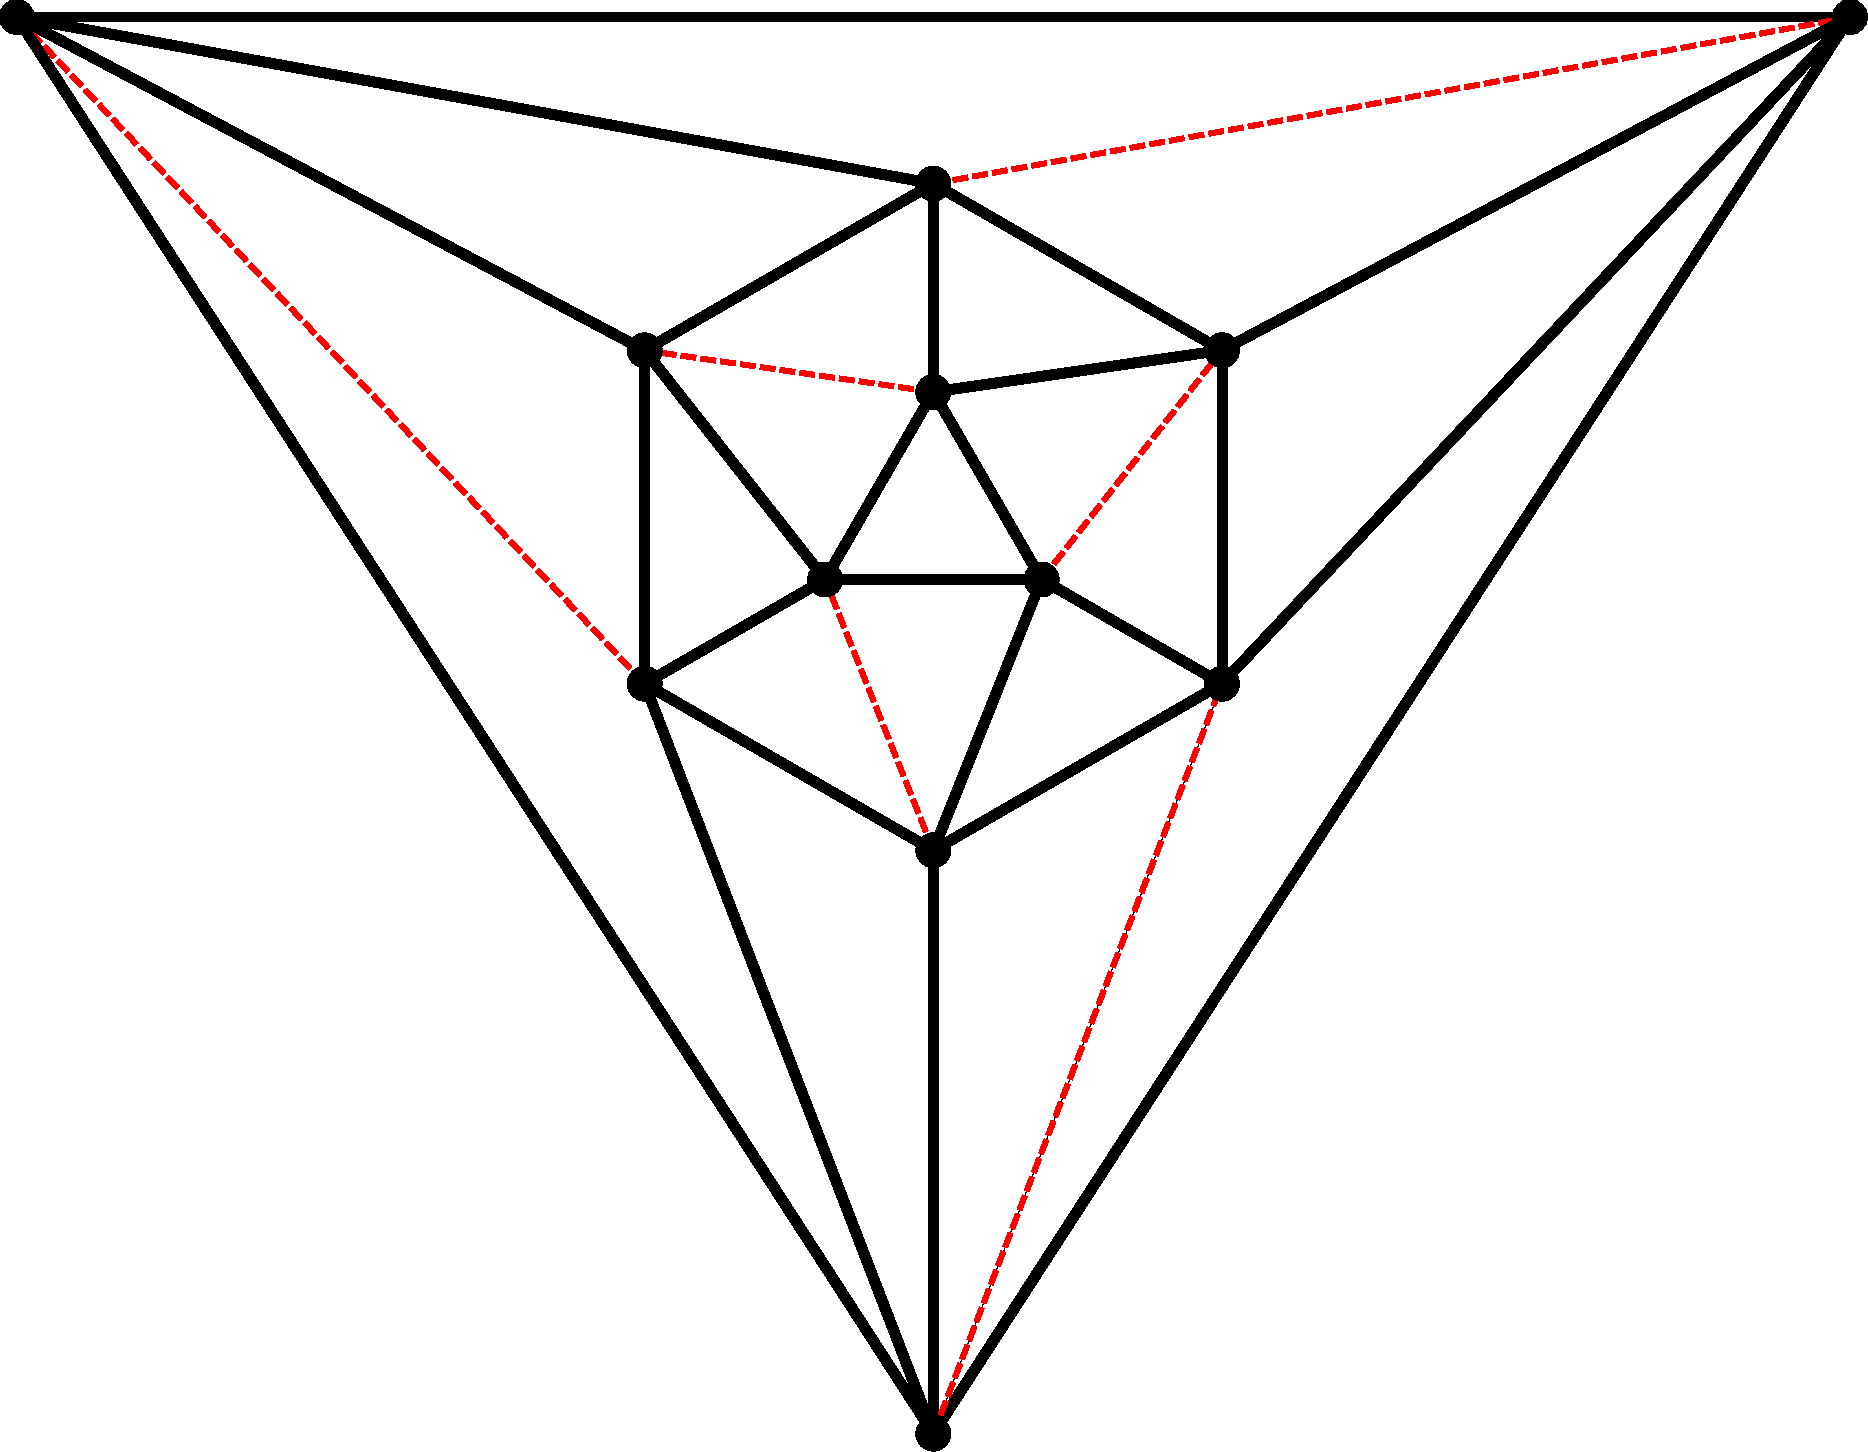
\includegraphics[width=0.3\textwidth]{gregory-newton/fcc.pdf}}\hspace{0.03\textwidth}
    \subfloat[hcp, $E=24$.\label{subfig:hcpgraph}]{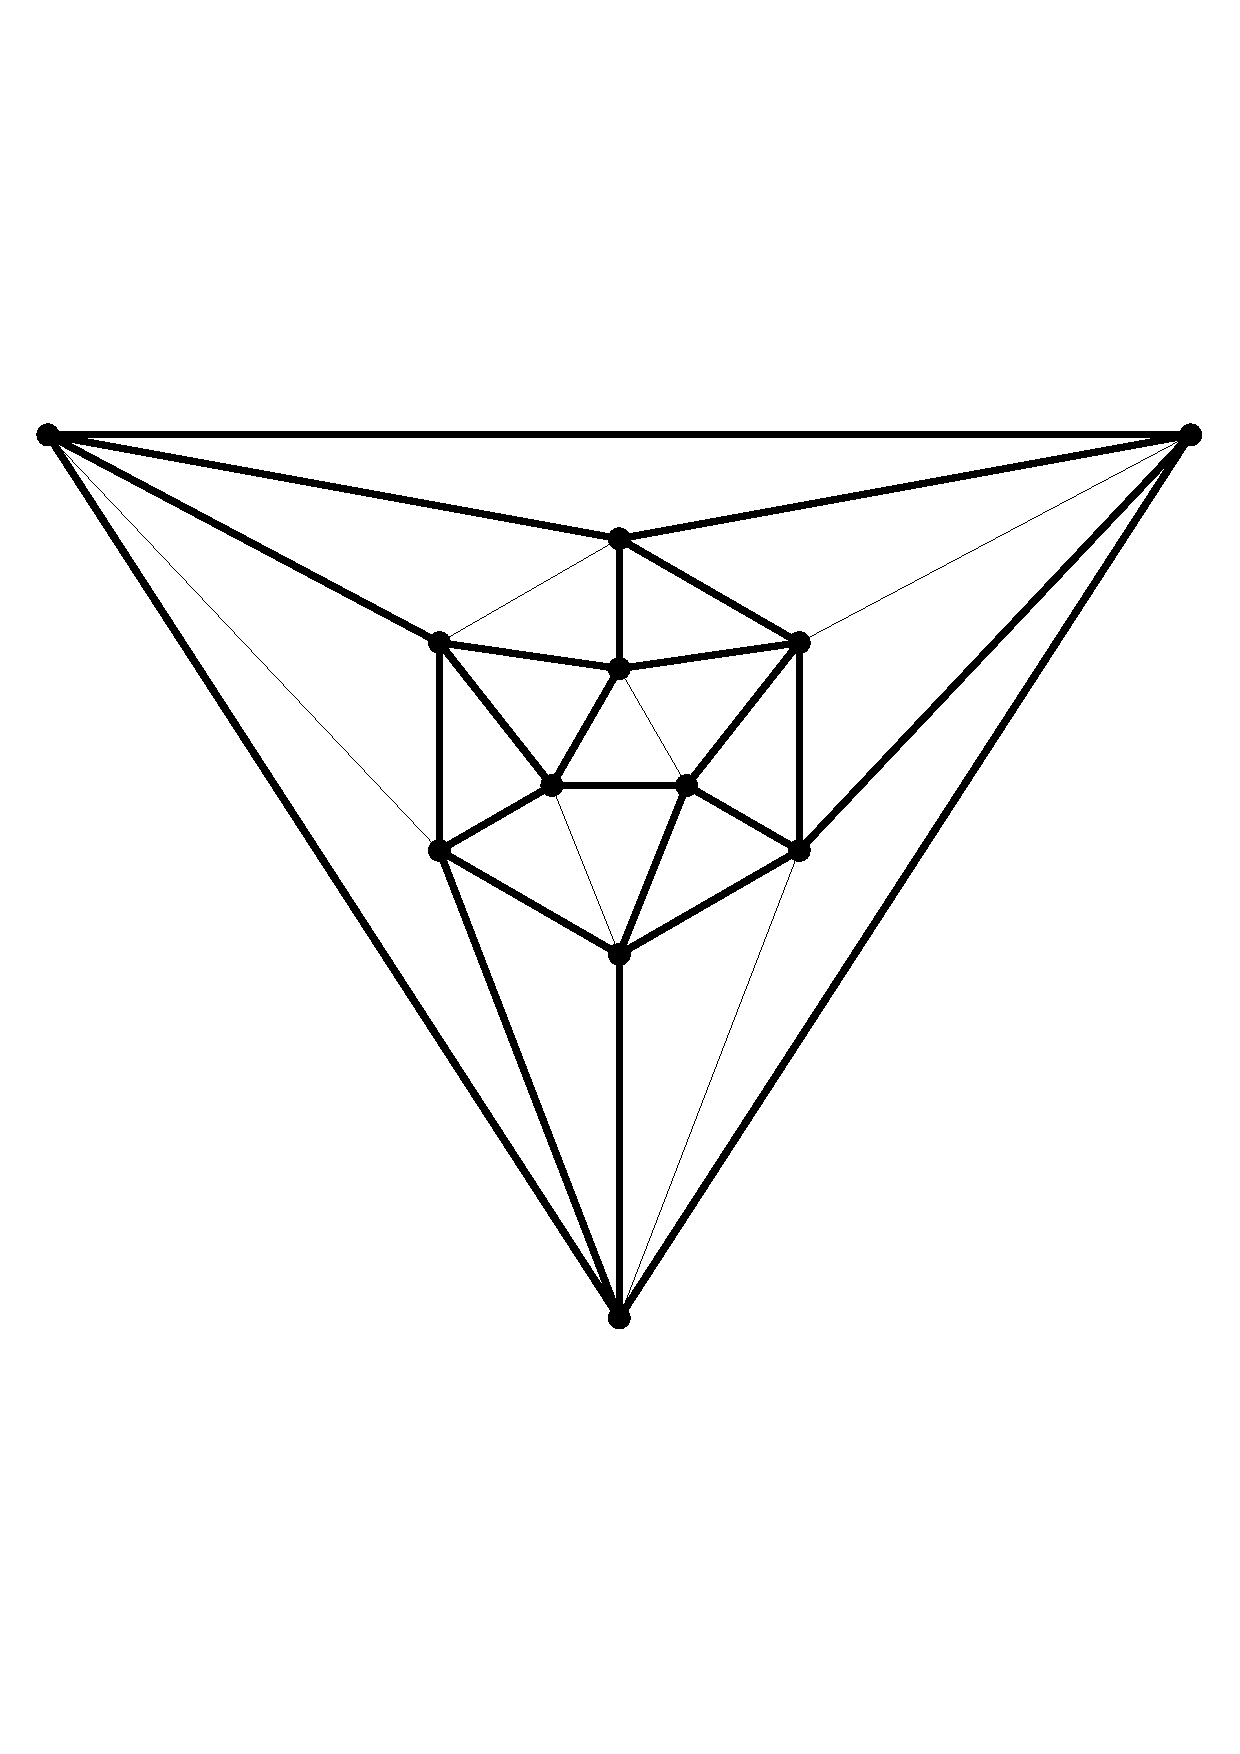
\includegraphics[width=0.3\textwidth]{gregory-newton/hcp.pdf}}\hspace{0.03\textwidth}
    \subfloat[Johnson solid, $E=23$.\label{subfig:johnsongraph}]{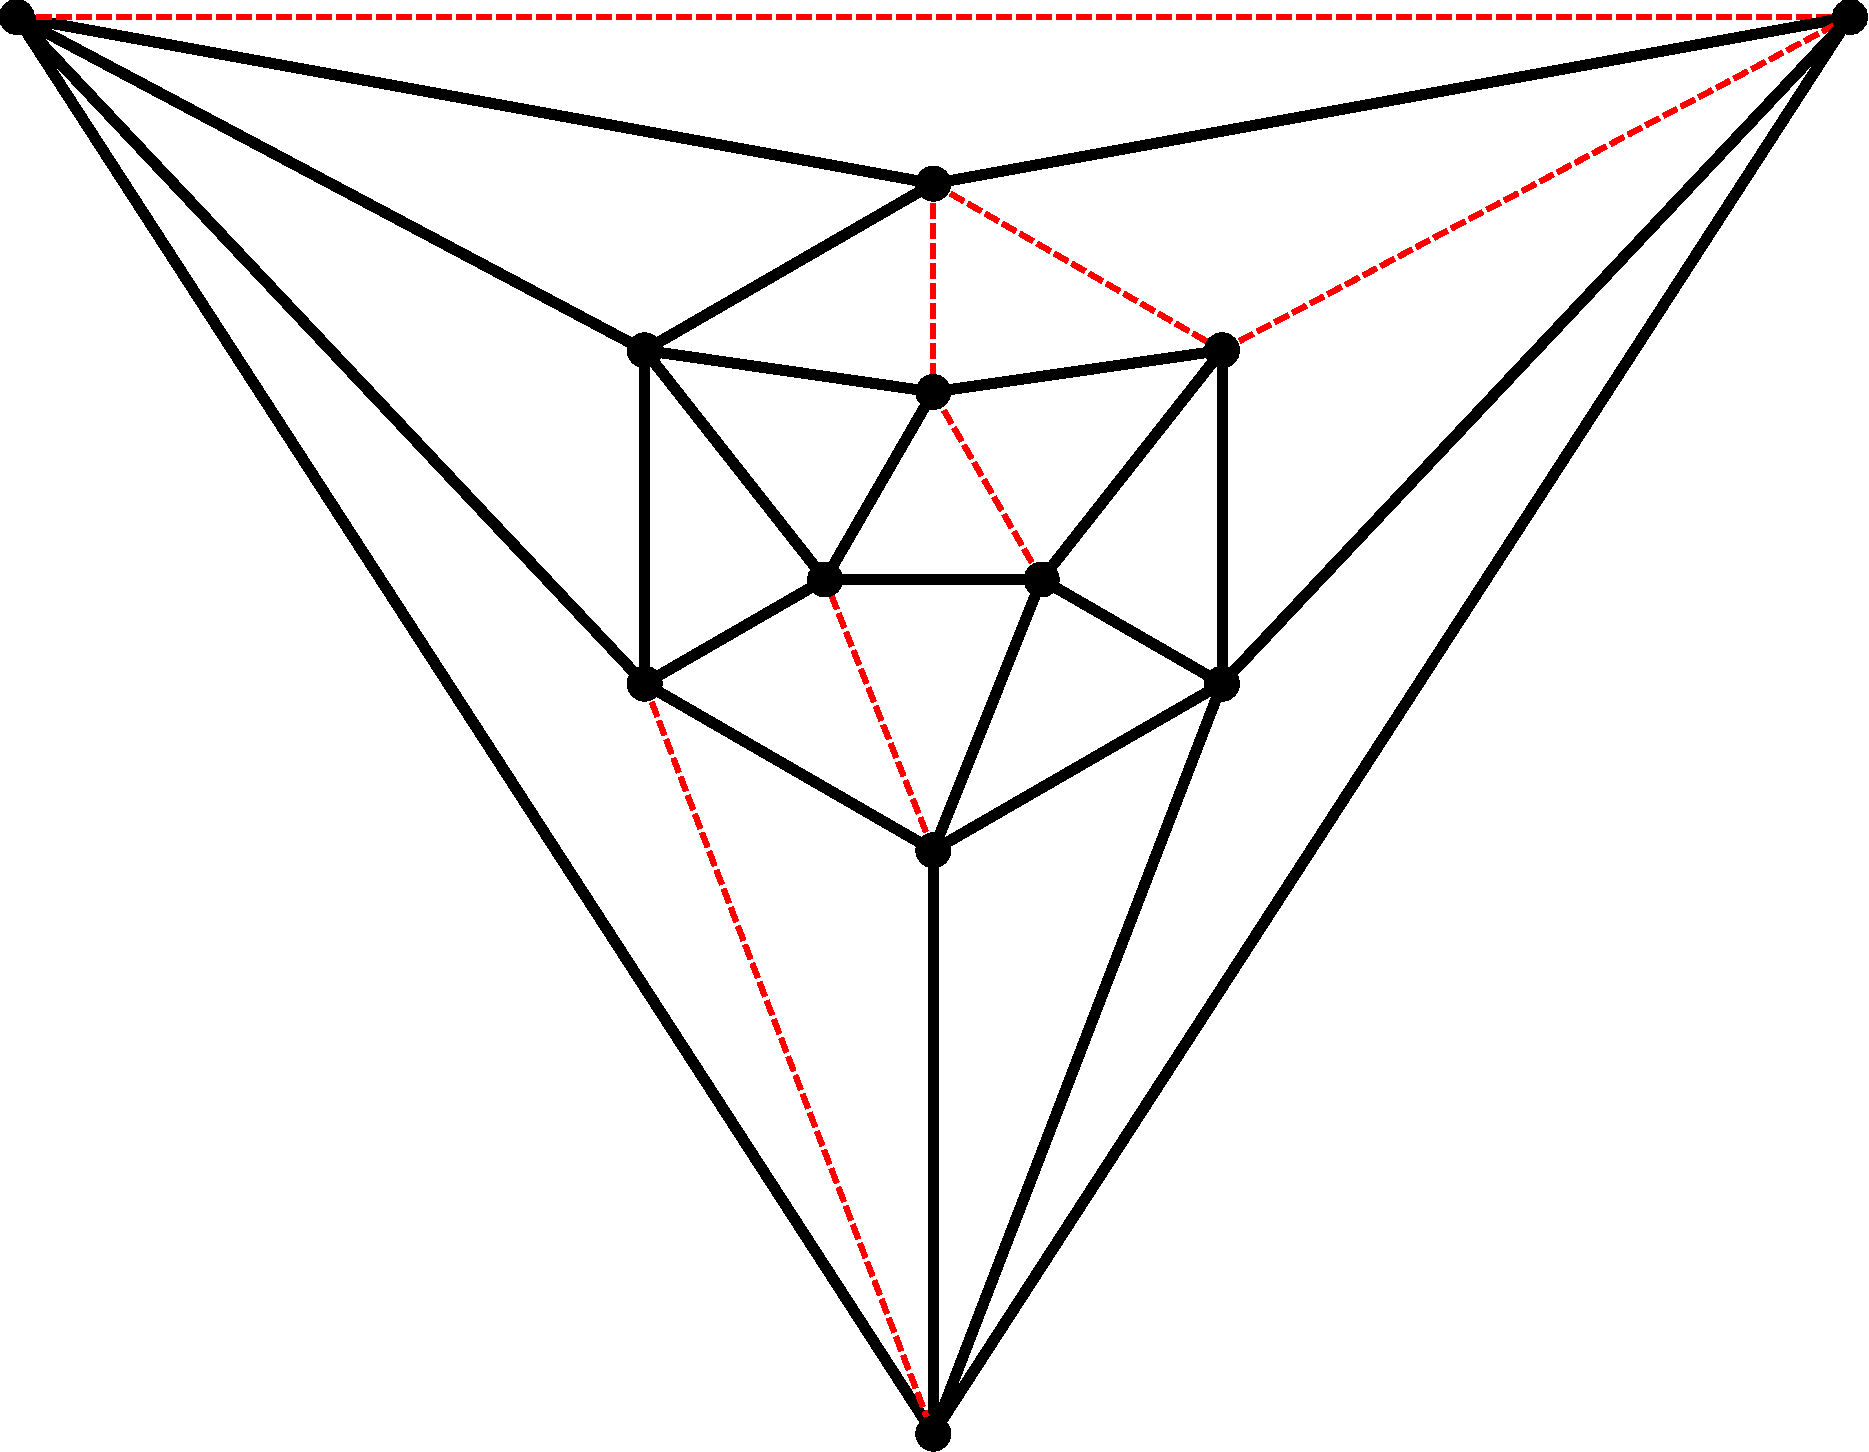
\includegraphics[width=0.3\textwidth]{gregory-newton/johnson.pdf}}
    \caption{Graphs of some \ac{GN} clusters mapped onto the icosahedral graph.
    Red lines indicate the edges that were removed to create the \ac{GN}
    cluster shell.}
    \label{fig:GNshellgraphs}
\end{figure}

Removing edges in this way means the resulting graphs only consists of
triangles and rectangles. The difference between the \ac{fcc} and hcp clusters
is in the way their square faces are connected. In \ac{fcc} the square faces
only connect via edges, while in hcp the square faces come in pairs sharing one
edge. 

These two cluster structures are the only possible ones when removing only six
edges. The reason for this can be explained by examining the structure of the
13-sphere Mackay icosahedron with respect to the limitations of the \ac{SHS}
potential. There are six $C_6$ symmetry axis in the $I_h$ point group. In the
ideal Mackay icosahedron there are pentagonal bipyramid motifs aligned along
those axis such that one of the tips coincides with the central atom and the
other tip becomes part of the 12-sphere shell (figure~\ref{fig:icopent}). 

\begin{figure}
    \centering
    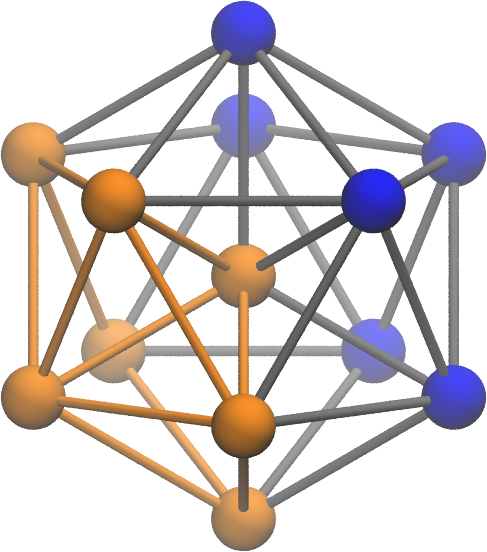
\includegraphics[width=.4\textwidth]{gregory-newton/icopent.png}
    \caption{13-sphere Mackay icosahedron. Orange spheres and bonds highlight
    the pentagonal bipyramid motif.}
    \label{fig:icopent}
\end{figure}

The pentagonal bipyramid is a structural motif that can't be realised under
\ac{SHS} conditions. This can be explained by looking at the motif as being
composed of five tetrahedra glued together at their faces. Ideal tetrahedra
can't be combined in this way as two vertices of the tetrahedra have to lose
contact.\autocite{Hayes_ScienceStickySpheres_2012} One can choose to either
break this connection between the tips of the bipyramid of between two vertices
of the pentagonal ring. In the \ac{GN} clusters this choice is restricted by
the fact that the connection between the tips of the bipyramid can't be broken
as this is one of the 12 \ac{COS} contact points.  This only leaves the choice
of breaking one bond of the pentagonal ring, which has to happen once for every
$C_6$ axis. The only possible solutions to this lead to the two closed-packed
clusters.

Removing one more edge yields only one possible \ac{GN} cluster with a shell
resembling an elongated pentagonal bipyramid
(figure~\ref{subfig:johnsongraph}). It consists of four edge-connected square
faces, a hexagonal face connecting the square faces and triangular faces.

There are 10 nonisomorphic structures if eight edges are removed, but the
majority of \ac{GN} clusters result from the removal of the maximum of nine
edges.


\subsection{Adding a 14th Sphere}
\label{sec:addinga14thsphere}

An even larger number of clusters exists for $N=14$ ($14529$), which is
$\approx 0.016|\mathcal{M}_\mathrm{SHS}(14)|$. All of these structures optimise
to just one of two possible (6,12)-LJ minima of \ac{GN} type. The first is the
Mackay icosahedron capped at one of its triangular faces, and the second is an
elongated pentagonal bipyramid (belonging to the class of Johnson solids) with
the 14th sphere capping a square face.

Most of these $N=14$ clusters are minimally rigid ($N_c=3N-6=36$), while only a
few are hyperstatic ($N_c > 3N-6$) and none are hypostatic ($N_c < 3N-6$).
There are $\{14369,144,8,6,2\}$ such clusters with $N_c=\{36,37,38,39,40\}$ and
$N=14$.  The clusters with $N_c=40$ are hcp and \ac{fcc} core-shell structures
capped at a square face; these arrangements maximise $N_c$. Most of the
clusters with $N_c=\{38,39\}$ are deformed versions of the elongated pentagonal
bipyramid mentioned above, indicating that this arrangement is a favoured route
to these intermediate-energy structures.  However, $N_c=39$ also contains hcp
and \ac{fcc} structures capped at a triangular face.  The first example of a cluster
derived from a perfect icosahedral symmetry shows up at lower value $N_c=37$
(!).  Representative examples for clusters with high contact numbers are
depicted in Figure~\ref{fig:N14}.  

\begin{figure}
    \centering
    \subfloat[$r_{14}^\text{GN}=1.34715$, $N_c=39$\label{subfig:short-greg-newton}]{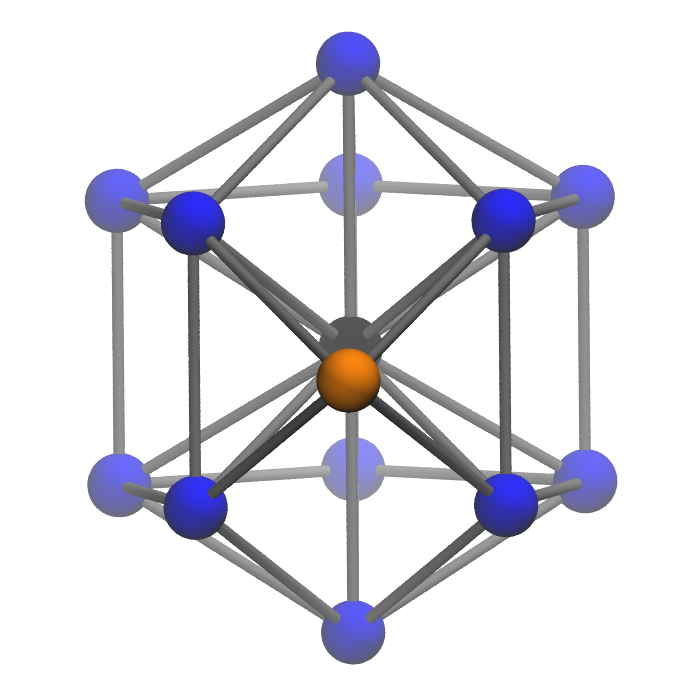
\includegraphics[width=0.4\textwidth]{gregory-newton/short.png}}
    \subfloat[$r_{14}^\text{GN}=1.37515$, $N_c=36$\label{subfig:2ndshort-greg-newton}]{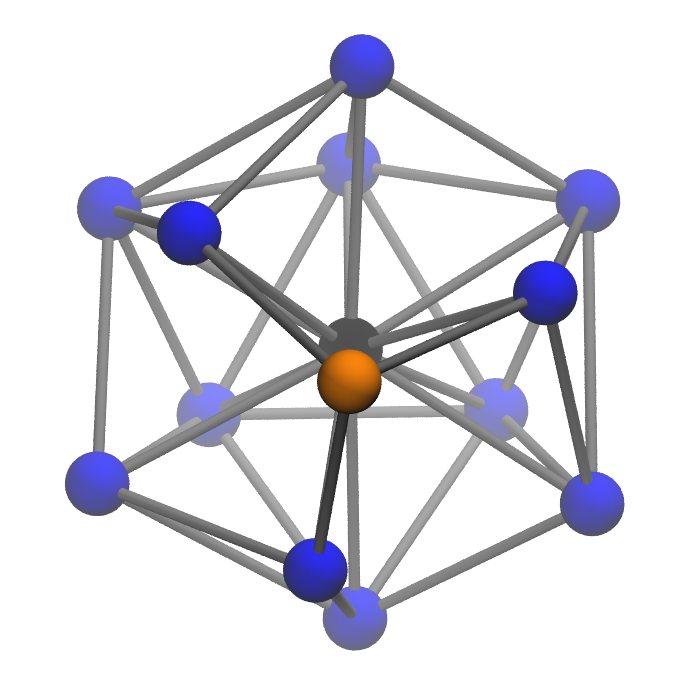
\includegraphics[width=0.4\textwidth]{gregory-newton/2ndshort.png}}\\
    \subfloat[$r_{14}^\text{GN}=\sqrt{2}$, $N_c=40$\label{subfig:sqrt2-greg-newton}]{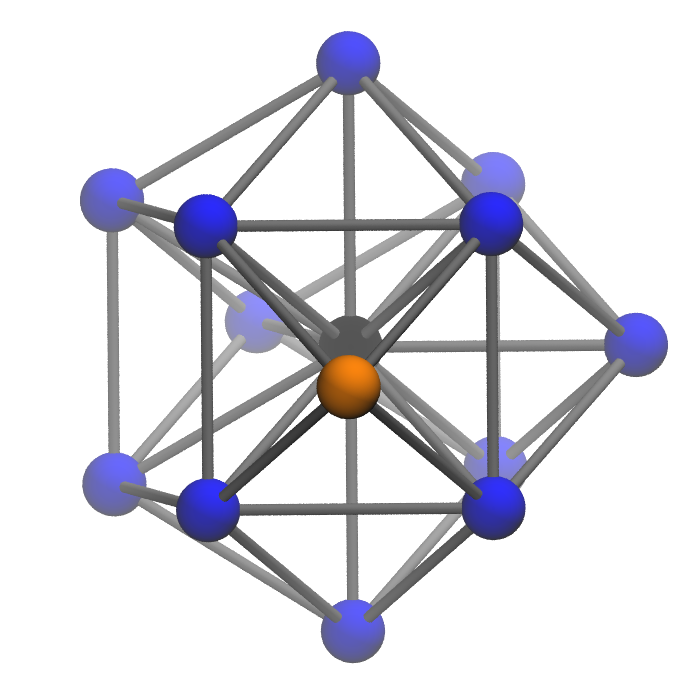
\includegraphics[width=0.4\textwidth]{gregory-newton/sqrt2.png}}
    \subfloat[$r_{14}^\text{GN}=\sqrt{\frac{8}{3}}$, $N_c=39$\label{subfig:sqrt83-greg-newton}]{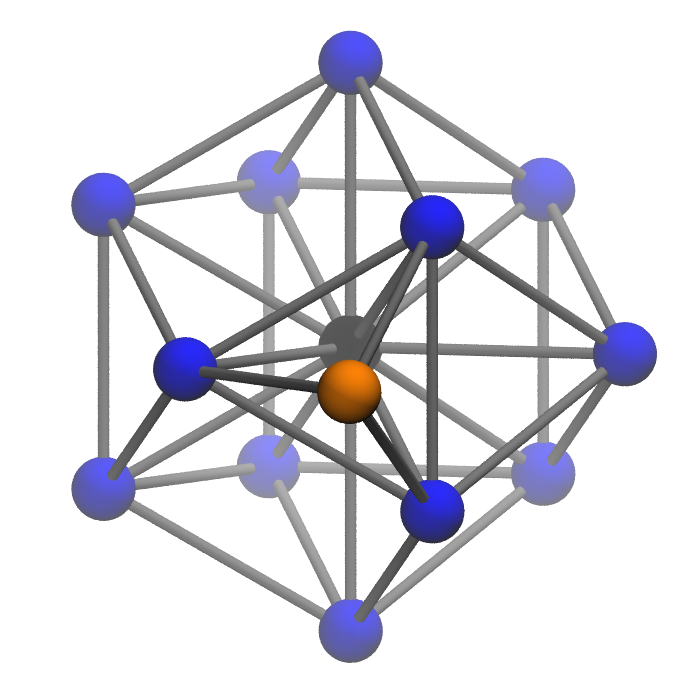
\includegraphics[width=0.4\textwidth]{gregory-newton/sqrt83.png}}\\
    \caption{Graphical representations of SHS packings with $N=14$, where a
center sphere is maximally contacting. The orange sphere in each cluster is the
14th outer sphere, not able to touch the center sphere (in black).  (a)
distorted elongated pentagonal bipyramid (Johnson solid); (b) distorted
icosahedron; (c) hcp capped on a square; (d) hcp capped on a triangle.}
    \label{fig:N14}
\end{figure}

\begin{figure}
    \centering
    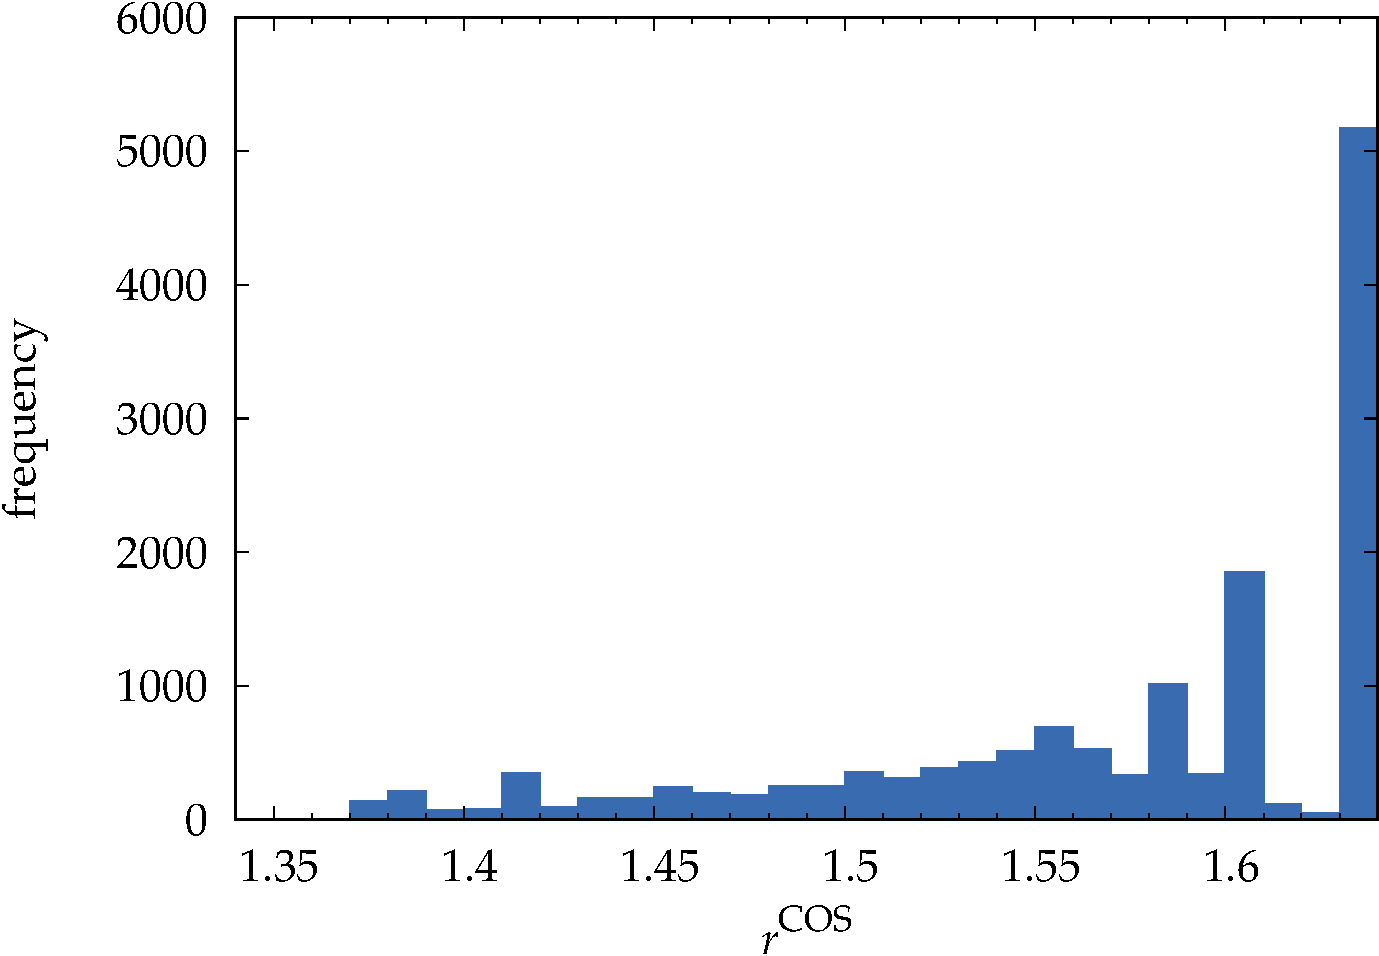
\includegraphics[width=0.8\textwidth]{gregory-newton/greg-newton.pdf}
    \caption{Frequency of distances from the cluster center to the most distant
    sphere for all Gregory-Newton-like clusters contained in the structures
    from Ref.~\cite{Holmes-Cerfon_EnumeratingRigidSphere_2016}. The width of the bars is $0.01$.}
    \label{fig:greg-newton}
\end{figure}


Surprisingly, the $N = 14$ cluster with the closest central-to-outer sphere
(COS) distance $r_\text{min}^\text{COS}$ was not known. Here we close this gap by
determining the COS distance for all Gregory-Newton type clusters.  We find one
single cluster with $r_\text{min}^\text{COS}=1.3471506281091$.  Its structure
(Fig.\ \ref{subfig:short-greg-newton}) is similar to the elongated pentagonal bipyramid (a
Johnson solid) with one of the square faces stretched to form a regular
rectangle.  The 14th sphere caps this deformed face, becoming the vertex of a
deformed octahedron and allowing the outer sphere to get closer to the central
sphere.  The next-smallest-$r^\text{COS}$ cluster ($r^\text{COS} = 1.37515$) is
shown in Fig.~\ref{subfig:2ndshort-greg-newton}.  It does not belong to the
category of the clusters derived from the elongated pentagonal bipyramid, but
instead can be described as being icosahedral-like.  The short distance is
achieved by attaching the 14th sphere to 3 spheres that do not form a face of
the cluster (because they are separated by a distance larger than $1$.)


As shown in Figure \ref{fig:greg-newton}, the distribution of $r^\text{COS}$
values for the full set of \ac{GN} clusters is shown in Figure
\ref{fig:greg-newton}.  Motifs with larger $r^\text{COS}$ are far more
prevalent.  For example, the peak at $r^\text{COS} = 1.41$ corresponds to
structures where the 14th sphere is touching 4 other spheres that are part of a
tetragonal pyramid, therefore forming a regular octahedron with a tip-to-tip
distance of $\sqrt{2}$ (Fig.~\ref{subfig:sqrt2-greg-newton}).  The maximum
$r^\text{COS}$ value ($1.63$) corresponds to capping triangular faces, so that
the most distant sphere is part of a regular trigonal bipyramid with a height
of $\sqrt{8/3}$ (Fig.~\ref{subfig:sqrt83-greg-newton}).  The structures in the
bars at $1.60,1.58$ and $1.55$ are derived from the regular trigonal bipyramid
and result from breaking its axial bonds.  In these structures, the more bonds
are broken, or the further the axial spheres are separated, the shorter the
center-to-outer sphere distance becomes.
